\documentclass[sigconf,anonymous,review]{acmart}
\usepackage{hyperref}
\usepackage{popets}

%\usepackage{amsmath,amssymb,amsfonts,bm}
\usepackage{bm}
%\usepackage{graphicx}

\usepackage{pgfplots}
\usepackage{acronym}
\usepackage{algorithm}
\usepackage{algpseudocode}
\usepackage{multirow}
\usepackage{tabularx}
%\usepackage{enumitem}
%\usepackage[e]{esvect}
\usepackage{subcaption}
%\usepackage{comment}
\usepackage[perpage]{footmisc}
\usepackage{cleveref}
\usepackage{enumitem}

% Copyright
\setcopyright{popets}
\copyrightyear{YYYY}

% Issue info
\acmYear{YYYY}
\acmVolume{YYYY}
\acmNumber{X}
\acmDOI{XXXXXXX.XXXXXXX}
\acmISBN{}
\acmConference{Proceedings on Privacy Enhancing Technologies}
\settopmatter{printacmref=false,printccs=false,printfolios=true}



\newcommand*\BitAnd{\mathbin{\&}}
\newcommand*\BitOr{\mathbin{|}}
\newcommand*\ShiftLeft{\ll}
\newcommand*\ShiftRight{\gg}
\newcommand*\RotateLeft{\lll}
\newcommand*\RotateRight{\ggg}
\newcommand*\BitNeg{\ensuremath{\mathord{\sim}}}


%\newcommand{\enc}[1]{\overline{#1}}
%\newcommand{\v}[1]{\mathbb{#1}}
%\newcommand{\encv}[1]{\overline{\mathbf{#1}}}


\newcommand{\kw}[1]{\textsf{#1}}
\newcommand{\bkw}[1]{\textsf{\textbf{#1}}}

\newcommand{\PSM}{\overline{\bkw{PSM}}}

\newcolumntype{C}{@{\extracolsep{8pt}}c@{\extracolsep{0pt}}}%
\newcolumntype{R}{@{\extracolsep{8pt}}r@{\extracolsep{4pt}}}%

%\newcolumntype{M}{@{\tabcolsep{3pt}}m{2pt}}%
\newcolumntype{M}[1]{>{\centering\let\newline\\\arraybackslash\hspace{0pt}}m{#1}}


\pgfplotsset{compat=1.18}



%footnotes
%\renewcommand{\thefootnote}{\fnsymbol{footnote}}
\renewcommand{\thefootnote}{\fnsymbol{footnote}}

% Maths
%Polynomials
\newcommand{\pa}{\mathbf{a}} % arbitrary polynomials
\newcommand{\pb}{\mathbf{b}}
\newcommand{\pc}{\mathbf{c}}
\newcommand{\pd}{\mathbf{d}}
\newcommand{\pe}{\mathbf{e}}
\newcommand{\pf}{\mathbf{f}}
\newcommand{\pg}{\mathbf{g}}
\newcommand{\ph}{\mathbf{h}}
\newcommand{\pj}{\mathbf{j}}
\newcommand{\pl}{\mathbf{l}}
\newcommand{\ppm}{\mathbf{m}}
\newcommand{\pn}{\mathbf{n}}
\newcommand{\po}{\mathbf{o}}
\newcommand{\pp}{\mathbf{p}}
\newcommand{\pq}{\mathbf{q}}
\newcommand{\pr}{\mathbf{r}}
\newcommand{\ps}{\mathbf{s}}
\newcommand{\pu}{\mathbf{u}}
\newcommand{\pvv}{\mathbf{v}}
\newcommand{\pw}{\mathbf{w}}
\newcommand{\px}{\mathbf{x}}
\newcommand{\py}{\mathbf{y}}
\newcommand{\pz}{\mathbf{z}}
\newcommand{\pA}{\mathbf{A}} % arbitrary matrix polynomials
\newcommand{\pB}{\mathbf{B}}
\newcommand{\pC}{\mathbf{C}}
\newcommand{\pD}{\mathbf{D}}
\newcommand{\pE}{\mathbf{E}}
\newcommand{\pF}{\mathbf{F}}
\newcommand{\pG}{\mathbf{G}}
\newcommand{\pH}{\mathbf{H}}
\newcommand{\pJ}{\mathbf{J}}
\newcommand{\pL}{\mathbf{L}}
\newcommand{\pM}{\mathbf{M}}
\newcommand{\pN}{\mathbf{N}}
\newcommand{\pO}{\mathbf{O}}
\newcommand{\pP}{\mathbf{P}}
\newcommand{\pQ}{\mathbf{Q}}
\newcommand{\pR}{\mathbf{R}}
\newcommand{\pS}{\mathbf{S}}
\newcommand{\pU}{\mathbf{U}}
\newcommand{\pV}{\mathbf{V}}
\newcommand{\pW}{\mathbf{W}}
\newcommand{\pX}{\mathbf{X}}
\newcommand{\pY}{\mathbf{Y}}
\newcommand{\pZ}{\mathbf{Z}}
\newcommand{\p}[1]{\bm{#1}}

%Vectors
\newcommand{\va}{\vv{a}} % arbitrary vectors
\newcommand{\vb}{\vv{b}}
\newcommand{\vc}{\vv{c}}
\newcommand{\vd}{\vv{d}}
\newcommand{\ve}{\vv{e}}
\newcommand{\vf}{\vv{f}}
\newcommand{\vg}{\vv{g}}
\newcommand{\vh}{\vv{h}}
\newcommand{\vi}{\vv{i}}
\newcommand{\vj}{\vv{j}}
\newcommand{\vk}{\vv{k}}
\newcommand{\vl}{\vv{l}}
\newcommand{\vm}{\vv{m}}
\newcommand{\vn}{\vv{n}}
\newcommand{\vo}{\vv{o}}
\newcommand{\vp}{\vv{p}}
\newcommand{\vq}{\vv{q}}
\newcommand{\vr}{\vv{r}}
\newcommand{\vs}{\vv{s}}
\newcommand{\vt}{\vv{t}}
\newcommand{\vu}{\vv{u}}
\newcommand{\vvv}{\vv{v}}
\newcommand{\vw}{\vv{w}}
\newcommand{\vx}{\vv{x}}
\newcommand{\vy}{\vv{y}}
\newcommand{\vz}{\vv{z}}
\newcommand{\0}{\vv{0}}  % The zero vector
\newcommand{\1}{\vv{1}}  % The vector of ones



\newcommand{\pv}[1]{\vv{\bm{#1}}}%%
\newcommand{\enc}[1]{\mathcal{E}\left({#1}\right)}
\newcommand{\senc}[2]{\mathcal{E}_{#2}\left({#1}\right)}


\newcommand{\cd}[1]{\vv{\sigma}(#1)}
\newcommand{\cdv}[1]{\vv{\sigma}(\pv{#1})}


%\newcommand{\encv}[1]{\mathcal{E}({\vv{\mathbf{#1}}})}
\newcommand{\encv}[1]{\mathcal{E}(#1)}%
%Matrices
\newcommand{\mA}{\mathbf{A}} % arbitrary vectors
\newcommand{\mB}{\mathbf{B}}
\newcommand{\mC}{\mathbf{C}}
\newcommand{\mD}{\mathbf{D}}
\newcommand{\mE}{\mathbf{E}}
\newcommand{\mF}{\mathbf{F}}
\newcommand{\mG}{\mathbf{G}}
\newcommand{\mH}{\mathbf{H}}
\newcommand{\mI}{\mathbf{I}} %identity matrix
\newcommand{\mJ}{\mathbf{J}}
\newcommand{\mK}{\mathbf{K}}
\newcommand{\mL}{\mathbf{L}}
\newcommand{\mM}{\mathbf{M}}
\newcommand{\mN}{\mathbf{N}}
\newcommand{\mO}{\mathbf{O}}
\newcommand{\mP}{\mathbf{P}}
\newcommand{\mQ}{\mathbf{Q}}
\newcommand{\mR}{\mathbf{R}}
\newcommand{\mS}{\mathbf{S}}
\newcommand{\mSigma}{\mathbf{\Sigma}}
\newcommand{\mT}{\mathbf{T}}
\newcommand{\mU}{\mathbf{U}}
\newcommand{\mV}{\mathbf{V}}
\newcommand{\mW}{\mathbf{W}}
\newcommand{\mX}{\mathbf{X}}
\newcommand{\mY}{\mathbf{Y}}
\newcommand{\mZ}{\mathbf{Z}}

%functions over vectors and matrices
\newcommand{\proj}{\pi}
\newcommand{\transpose}[1]{#1^{\intercal}} %transpose
\newcommand{\inprod}[2]{\langle #1, #2 \rangle} %inner product
\newcommand{\Tr}{\mathrm{Tr}} %trace
\newcommand{\TrOf}[1]{\Tr\!\left(#1\right)}
\newcommand{\No}{\mathrm{No}} %norm

%numerical sets
\newcommand{\Z}{\mathbb{Z}} %integers
\newcommand{\N}{\mathbb{N}} %natural numbers
\newcommand{\Q}{\mathbb{Q}} %rational numbers
\newcommand{\R}{\mathbb{R}} %real numbers
\newcommand{\C}{\mathbb{C}} %complex numbers
\newcommand{\F}{\mathbb{F}} %finite field
\newcommand{\K}{\mathcal{K}} %arbitrary set
\renewcommand{\S}{\mathcal{S}} %arbitrary set
\newcommand{\D}{\mathcal{D}} %Random Distribution
\newcommand{\U}{\mathcal{U}} %Uniform Distribution
\newcommand{\T}{\mathcal{T}} %Ternary Distribution
\newcommand{\A}{\mathcal{A}} %Adversary
\newcommand{\B}{\mathcal{B}} %Simulator

%complex numbers
\newcommand{\conj}[1]{\overline{#1}}

%special constants
\newcommand{\iu}{{i\mkern1mu}} %imaginary i

%ideals
\newcommand{\ideal}[1]{\left\langle #1 \right\rangle}
\newcommand{\idealI}{\mathcal{I}}
\newcommand{\idealJ}{\mathcal{J}}
\newcommand{\idealp}{\mathfrak{p}}

\newcommand{\idealNormOf}[1]{N\!\left(#1\right)}

%sets
\newcommand{\cardinOf}[1]{\left\lvert#1\right\rvert}

\DeclareMathSymbol{\shortminus}{\mathbin}{AMSa}{"39}


%arithmetic functions
\newcommand{\mult}{{\mathrm{mult}}}
\newcommand{\mul}{{\mathrm{mul}}}
\newcommand{\add}{{\mathrm{add}}}
\newcommand{\erf}{{\mathrm{erf}}}
\newcommand{\erfc}{{\mathrm{erfc}}}
\newcommand{\inv}[1]{{#1}^{\!\shortminus1}}
%\newcommand{\inv}[1]{{{#1}^{-1}}}

%size
\newcommand{\size}{{\mathrm{size}}}

%probability
\newcommand{\Prob}{{\mathrm{Prob}}} % probability

%parameters of any generalized encryption scheme
\newcommand{\ctxtSpace}{\mathcal{C}} %ciphertext space
\newcommand{\ptxtSpace}{\mathcal{P}} %plaintext space
\newcommand{\msgSpace}{\mathcal{M}} %message space
\newcommand{\secpar}{\lambda} %security parameter

%elements of any encryption scheme
\newcommand{\sk}{{\mathtt{sk}}}
\newcommand{\pk}{{\mathtt{pk}}}
\newcommand{\rlk}{{\mathtt{rlk}}}
\newcommand{\ct}{{\mathtt{ct}}}
\newcommand{\pt}{{\mathtt{pt}}}

%basic encryption operations
\newcommand{\KeyGen}{{\mathtt{KeyGen}}}
\newcommand{\SKGen}{{\mathtt{SecretKeyGen}}}
\newcommand{\PKGen}{{\mathtt{PublicKeyGen}}}
\newcommand{\EVGen}{{\mathtt{EvaluateKeyGen}}}
\newcommand{\RKGen}{{\mathtt{RelinKeyGen}}}
\newcommand{\BKGen}{{\mathtt{BootKeyGen}}}
\newcommand{\Encrypt}{{\mathtt{Encrypt}}}
\newcommand{\Enc}{\mathtt{Enc}}
\newcommand{\Decrypt}{{\mathtt{Decrypt}}}
\newcommand{\Dec}{\mathtt{Dec}}
\newcommand{\Encode}{{\mathtt{Encode}}}
\newcommand{\Decode}{{\mathtt{Decode}}}
\newcommand{\Pack}{{\mathtt{Pack}}}
\newcommand{\Unpack}{{\mathtt{Unpack}}}

\newcommand{\TrapGen}{\bkw{TrapGen}}
\newcommand{\SamplePre}{\bkw{SamplePre}}
\newcommand{\PRGN}{\bkw{PRGN}}
\newcommand{\PRF}{\bkw{PRF}}
\newcommand{\RSIS}{\bkw{RSIS}}


%homomorphic encryption operations
\newcommand{\Add}{{\mathtt{Add}}}
\newcommand{\AddPlain}{{\mathtt{AddPlain}}}
\newcommand{\Sub}{{\mathtt{Sub}}}
\newcommand{\SubPlain}{{\mathtt{SubPlain}}}
\newcommand{\BasicMul}{{\mathtt{BasicMul}}}
\newcommand{\Mul}{{\mathtt{Mul}}}
\newcommand{\MulPlain}{{\mathtt{MulPlain}}}
\newcommand{\ModSwitch}{{\mathtt{ModSwitch}}}
\newcommand{\Relin}{{\mathtt{Relin}}}
\newcommand{\Rescale}{{\mathtt{Rescale}}}
\newcommand{\Rotate}{{\mathtt{Rot}}}
\newcommand{\Shift}{{\mathtt{Shift}}}
\newcommand{\Frob}{{\mathtt{Frob}}}
\newcommand{\Eval}{{\mathtt{Evaluate}}}
\newcommand{\Select}{{\mathtt{Select}}}
\newcommand{\Replicate}{{\mathtt{Replicate}}}
\newcommand{\IsNonZero}{{\mathtt{IsNonZero}}}
\newcommand{\Power}{{\mathtt{IsNonZero}}}

%lattices
\newcommand{\lat}{\mathcal{L}}
\newcommand{\mindist}{{\lambda_1}}
\newcommand{\mindistOf}[1]{{\lambda_1}\!\left(#1\right)}
\newcommand{\sucmin}[1]{{\lambda_#1}}
\newcommand{\sucminOf}[2]{{\lambda_#1}\!\left(#2\right)}
\newcommand{\smoothpar}[1]{{\eta_#1}}
\newcommand{\smoothparOf}[2]{{\eta_#1}\!\left(#2\right)}
\newcommand{\duallat}[1]{{#1^*}}

%number theory
\newcommand{\numfield}{\mathcal{K}} %the number field 
\newcommand{\numfieldDim}{n} %the dimension of the number field over the field of rational numbers
\newcommand{\defpoly}{f} %the definining polynomial of the number field
\newcommand{\intring}{\mathit{R}} %the ring of integers of a number field
\newcommand{\expfactor}{\delta_{\mathcal{R}}} %expansion factor 
\newcommand{\dual}[1]{\ensuremath{#1^\vee}} %the dual of an ideal
\newcommand{\codifen}{\dual{\intring}}
\newcommand{\canemb}{\sigma} %canonical embedding
\newcommand{\canembMat}{\boldsymbol{\Sigma}} %linear operator of the canonical embedding
\newcommand{\invCanembMat}{\inv{\canembMat}} %invers of the linear operator of the canonical embedding
\newcommand{\canembImg}{H} %image of the canonical embedding in the complex vector space
\newcommand{\canembImgBasis}{\mB} %basis of the can. embedding image over real numbers
\newcommand{\realembNum}{{s_1}} %number of real embeddings
\newcommand{\cmplxembNum}{{s_2}} %number of non-cojugate complex embeddings
\newcommand{\cyclpoly}[1]{{\Phi_{#1}}} %cyclotomic polynomial
\newcommand{\cyclpolyOrd}{m} %order of a cyclotomic polynomial
\newcommand{\CRT}{\mathsf{CRT}} %Chinese remainder theorem ring isomorphism
\newcommand{\disc}{\mathrm{disc}}
\newcommand{\ord}{{\mathrm{ord}}} %order of an element
\newcommand{\eulerphi}[1]{\phi\left(#1\right)} %Euler totient function
\DeclareMathOperator{\Gal}{Gal} %Galois group

\newtheorem{lemma}{Lemma}
%\newtheorem{theorem}{Theorem}
\newtheorem{definition}{Definition}

%lattice problems
\acrodef{BDD}{Bounded Distance Decoding}
\acrodef{SIS}{Short Integer Solution}
\acrodef{SVP}{Shortest Vector Problem}
\acrodef{uSVP}{Unique Shortest Vector Problem}
\acrodef{GapSVP}{Decision Shortest Vector Problem}
\acrodef{SIVP}{Shortest Independent Vectors Problem}
\acrodef{DGS}{Discrete Gaussian Sampling}
\acrodef{LWE}{Learning with Errors}
\acrodef{SLWE}{Search Learning with Errors}
\acrodef{DLWE}{Decision Learning with Errors}
\acrodef{S(I)VP}{Shortest (Independent) Vector Problem}
\acrodef{RLWE}{Ring Learning with Errors}
\acrodef{MLWE}{Module Learning with Errors}
\acrodef{RSIS}{Ring Short Integer Solution}
\acrodef{MSIS}{Module Short Integer Solution}

%lattice acronyms
\acrodef{ANF}{Algebraic Normal Form}
\acrodef{HNF}{Hermite Normal Form}

%LWE parameters
\newcommand{\LWEdim}{n}
\newcommand{\LWEmod}{q}

%RLWE parameters
\newcommand{\LWE}{\textsf{LWE}}
\newcommand{\RLWE}{\textsf{RLWE}}
\newcommand{\MLWE}{\textsf{MLWE}}
\newcommand{\SRLWE}{\textsf{S-RLWE}}
\newcommand{\DRLWE}{\textsf{D-RLWE}}
\newcommand{\RLWEbasicRing}{\intring}
\newcommand{\RLWEdim}{n}
\newcommand{\RLWEmod}{\LWEmod}
\newcommand{\RLWEring}{{\RLWEbasicRing_\RLWEmod}}
\newcommand{\SCGLWE}{\text{SCG}\textsf{-LWE}}

%HE names
\acrodef{HE}{Homomorphic Encryption}
\acrodef{FHE}{Fully Homomorphic Encryption}
\acrodef{SHE}{Somewhat Homomorphic Encryption}
\acrodef{LHE}{Leveled Homomorphic Encryption}
\acrodef{BGV}{Brakerski-Gentry-Vaikuntanathan}
\acrodef{FV}{Fan-Vercauteren}
\acrodef{GSW}{Gentry-Sahai-Waters}
\acrodef{HAO}{Hiromasa-Abe-Okamoto}
\acrodef{LTV}{Lopez-Tromer-Vaikuntanathan}
\acrodef{YASHE}{Yet Another Somewhat Homomorphic Encryption}
%\newcommand{\BCIV}{\mathtt{BCIV}}
%\newcommand{\HEAAN}{\mathtt{HEAAN}}
%\newcommand{\TFHE}{\mathtt{TFHE}}

%FHE/SHE names
\newcommand{\BGV}{\mathtt{BGV}}
\newcommand{\HEAAN}{\mathtt{HEAAN}}
\newcommand{\BFV}{\mathtt{BFV}}
\newcommand{\OTK}{\mathtt{OTK}}
\newcommand{\FV}{\mathtt{FV}}
\newcommand{\BCIV}{\mathtt{BCIV}}
\newcommand{\TFHE}{\mathtt{TFHE}}

%FV parameters
\newcommand{\FVringDim}{n}
\newcommand{\FVctxtMod}{\LWEmod}
\newcommand{\FVptxtMod}{t}
\newcommand{\FVDelta}{\Delta}
\newcommand{\FVrelinBase}{w}
\newcommand{\FVrlkNum}{\ell}
\newcommand{\FVctxtSpace}{\RLWEbasicRing_\FVctxtMod^2}
\newcommand{\FVptxtSpace}{\RLWEbasicRing_\FVptxtMod}
\newcommand{\slots}{\ell}

%BGV parameters
\newcommand{\BGVptxtMod}{t}

%HEAAN parameters
\newcommand{\HEAANscale}{\Delta}

%RNS operations
\newcommand{\FastBconv}{{\mathtt{FastBconv}}}

%message
\newcommand{\msg}{\mathsf{msg}}

%norms
\newcommand{\abs}[1]{\left\lvert #1 \right\rvert}
\newcommand{\norm}[1]{\left\lVert #1 \right\rVert}
\newcommand{\canorm}[1]{\left\lVert #1 \right\rVert^{\textup{can}}}
\newcommand{\infnorm}[1]{\left\lvert#1\right\rvert_\infty}

% various functions
\newcommand{\wt}{\texttt{wt}}
\DeclareMathOperator{\argmax}{argmax}
\DeclareMathOperator{\sign}{sgn}


%modular operation
\newcommand{\modq}[1]{\left[ #1 \right]_\RLWEmod} %modulo (R)LWE modulus in the symmetric interval
\newcommand{\modx}[2]{\left[ #2 \right]_{#1}} %modulo any modulus in the symmetric interval
\newcommand{\modp}[1]{\left[ #1 \right]_p} %modulo p in the symmetric interval
\newcommand{\modt}[1]{\left[ #1 \right]_\FVptxtMod} %modulo the FV plaintext modulus in the symmetric interval
\newcommand{\rem}[2]{\left| #2 \right|_{#1}} %remainder after division

%rounding operations
\newcommand{\round}[1]{\left\lfloor #1 \right\rceil} %rounding
\newcommand{\floor}[1]{\left\lfloor #1 \right\rfloor} %floor
\newcommand{\ceil}[1]{\left\lceil #1 \right\rceil} %ceiling

%distributions
\newcommand{\rand}{\xleftarrow{\$}} %sampled from (Vincent)
\newcommand{\from}{\leftarrow} %sampled from
\newcommand{\ufrom}{\xleftarrow{\$}} %sampled uniformly random from
\newcommand{\udist}{\mathcal{U}} %uniform distribution
\newcommand{\normdist}{\Gamma} %normal distribution
\newcommand{\dgaussdist}{\mathcal{DG}} %discrete Gaussian distribution
\newcommand{\keydist}{\chi_{\text{k}}} %key distribution
\newcommand{\errdist}{\chi_{\text{e}}} %error distribution
\newcommand{\stdev}{\sigma} %standard deviation

%indistinguishability of distributions
\newcommand{\cindist}{\stackrel{\rm c}{\approx}} %computational
\newcommand{\sindist}{\stackrel{\rm s}{\approx}} %statistical

%proof start/end
\newcommand{\bproof}{\noindent {\scshape Proof: }}
\newcommand{\eproof}{\ \mbox{} \hfill $\square$\mbox{}\newline}

%circuits
\newcommand{\circuit}{\mathcal{C}}

%boolean operators
\newcommand{\XOR}{\mathtt{XOR}}
\newcommand{\NAND}{\mathtt{NAND}}
\newcommand{\AND}{\mathtt{AND}}
\newcommand{\EQ}{\mathtt{EQ}}
\newcommand{\LT}{\mathtt{LT}}
\newcommand{\IsNegative}{\mathtt{IsNegative}}
\newcommand{\OR}{\mathtt{OR}}
\newcommand{\NOT}{\mathtt{NOT}}
\newcommand{\MOD}{\mathtt{MOD}}

%complexity classes
\newcommand{\poly}{\mathrm{poly}}

%technical commands
\newcommand{\remove}[1]{}
\newcommand{\alert}[1]{\textcolor{red}{#1}}

%comments
\newcommand{\que}[1]{{\color{red} {(\textbf{question:} #1})\xspace}}
\newcommand{\todo}[1]{\textcolor{red}{(TODO: #1)}}

%cryptographic acronyms
\acrodef{GC}{Garbled Circuit}
\acrodef{DSPR}{Decisional Small Polynomial Ratio}
\acrodef{FHE}{Fully Homomorphic Encryption}

%algorithmic acronyms
\acrodef{SVM}{Support Vector Machine}
\acrodef{LLL}{Lenstra Lenstra Lov{\'a}sz}
\acrodef{GMDH}{Group Method of Data Handling}

%math acronyms
\acrodef{CRT}{Chinese Remainder Theorem}
\acrodef{RNS}{Residue Number System}
\acrodef{NTT}{Number Theoretic Transform}
\acrodef{DFT}{Discrete Fourier Transform}

%computer science acronyms
\acrodef{SIMD}{Single Instruction Multiple Data}
\acrodef{SP}{Streaming Processor}
\acrodef{LSB}{Least Significant Bit}
\acrodef{CPU}{Central Processing Unit}
\acrodef{GPU}{Graphics Processor Unit}
\acrodef{SMP}{Symmetric Multiprocessing}
\acrodef{HPC}{High Performance Computing}
\acrodef{APU}{Accelerated Processing Unit}
\acrodef{FPGA}{Field-Programmable Gate Array}



\newcommand\blankfootnote[1]{%
  \begingroup
  \renewcommand\thefootnote{}\footnote{#1}%
  \addtocounter{footnote}{-1}%
  \endgroup
}
\newcommand*{\skipnumber}[2][1]{%
{\renewcommand*{\alglinenumber}[1]{}\State #2}%
\addtocounter{ALG@line}{-#1}}

\newcommand\SUM{\overline{\bkw{Sum}}}

%%% Local Variables:
%%% mode: latex
%%% TeX-master: "main"
%%% End:


\begin{document}

\title{Quantum-safe Anonymous Credentials from Homomorphic Encryption}

\author{Carlos Ribeiro}
\orcid{xxx}
\affiliation{%
  \institution{Instituto Superior Técnico}
  \city{Lisbon}
  \country{Portugal}}
\email{carlos.ribeiro@tecnico.ulisboa.pt}



\begin{abstract}
The growing emphasis on privacy, driven by the abundance of electronic data and advances in analytical and artificial intelligence tools, has been reinforced by recent legislation like GDPR and CCPA. Identity management systems (IMS) are at the heart of privacy concerns, facing challenges related to traceability and overdisclosure, both online and offline. Anonymous Credentials, introduced by D. Chaum in 1985, have gained prominence, but recent research is exploring new approaches, often based on lattice-based assumptions, to address quantum computing threats.

This proposal takes a unique approach by leveraging homomorphic encryption and verifiable decryption methods to protect attributes and demonstrate specific computations over signed attributes without full disclosure. It offers advantages in versatile attribute verification, reducing the need for additional credentials, and addressing revocation concerns while maintaining privacy.

The solution is built on three key primitives, including a verifiable decryption mechanism, a method to perform inequalities and private membership tests in homomorphic encryptions, and a variant of the GPV signature suitable for homomorphic verification.
\end{abstract}

\maketitle

\section{Introduction}
The focus on privacy has increased due to the vast amount of electronic data and advances in analytical and artificial intelligence tools. Recent legislation such as GDPR (General Data Protection Regulation) \cite{GDPR2016a} and CCPA (California Consumer Privacy Act) \cite{bukatyCaliforniaConsumerPrivacy2019} emphasize the need for strict transmission of private information. Identity management systems (IMS) are at the centre of this issue, as they must prove identity traits without leaking unnecessary information. Online IMS can have traceability problems, revealing the frequency of identifications and services contacted by individuals. Offline IMS, based on signed credentials, may transmit more information than necessary and can also have traceability issues when colluding with services.

The concept of Anonymous Credentials was first proposed by D. Chaun in 1985\cite{chaumSecurityIdentificationTransaction1985}, but it was not until 2001 that the first fully functional solution was proposed\cite{camenischEfficientSystemNontransferable2001}. Since then, there have been many different proposals targeting additional features\cite{laponAnalysisRevocationStrategies2011,garmanDecentralizedAnonymousCredentials2013,camenischEfficientAttributesAnonymous2012,connollyImprovedConstructionsAnonymous2022}, efficiency\cite{camenischAnonymousAttestationUsing2016a}, standardization\cite{curranAnonCredsSpecification2023}, and concrete implementations\cite{lodderAnonymousCredentials2019}. Recently, there has been a new line of research\cite{bootleFrameworkPracticalAnonymous2023,blazyEfficientImplementationPostQuantum2023,boschiniEfficientPostquantumSNARKs2020,jeudyLatticeSignatureEfficient2022,laiLatticebasedCommitTransferrableSignatures2023,boschiniRelaxedLatticeBasedSignatures2018} that aims to change the cryptographic assumptions used in these solutions, as current assumptions are believed to become obsolete with the advent of quantum computing. Most of the new proposed solutions for quantum-safe cryptography are based on lattice-based assumptions\cite{FIPS203,FIPS204}, but different strategies exist, using: (i) lattice-based zero-knowledge proof systems\cite{lyubashevskyLatticeBasedZeroKnowledgeProofs2022}, (ii) zkSNARKs\cite{boschiniEfficientPostquantumSNARKs2020}, or as in the present proposal, (iii) homomorphic encryption to prove attributes without complete disclosure. Each solution should be studied, improved, and compared with others to overcome its challenges.



Although most existing solutions rely on concealing credential attributes within signed commitments, which holders then selectively demonstrate to verifiers using zero-knowledge proofs, our approach takes a different route. We employ homomorphic encryption to shield these attributes and employ verifiable decryption methods to demonstrate the result of specific computations over signed attributes to verifiers, without disclosing the attributes.

This approach offers a significant advantage: it extends beyond the conventional boundaries of attribute disclosure. For instance, it can validate statements such as "older than 18" without divulging the precise birthdate or necessitating the issuance of additional credentials. Additionally, it can verify attributes such as "address is from an EU member state" by privately inferring this information from the member state's name in the address. Moreover, our solution can verify functions across attributes in various credentials from different issuers without requiring intermediate issuers to issue new credentials, which reduces the need for extensive interaction within the overall system.

Revocation is of paramount relevance in any solution with long-lived credentials. However, revocation is notably absent in many proposals. Our solution capitalizes on the expressiveness of our attribute-proof system to build a simple revocation mechanism that still preserves privacy.

The drawback of our proposal is the size of the credentials' presentations. While the credentials themselves can be less than $5KB$\footnote{Assuming that the holder knows the attributes the issuer only needs to send the signature.}, the presentations of the credentials (sent from the holder to the verifier) vary with the number of attributes and the depth of the function to be proved, which for the depth required by our comparison primitives (Section \ref{sec:comparison}) is $\approx734~KB$.

Our solution is based on three primitives that may be of independent interest: (i) a special verifiable decryption primitive, first suggested in \cite{chillottiHomomorphicLWEBased2016}; (ii) a primitive for performing simple inequalities and private membership tests in homomorphic encryptions; and (iii) a variant of the GPV signature that can be verified homomorphically.


\section{Related Work}
At its core\cite{lysyanskayaSignatureSchemesApplications2002}, anonymous credentials involve three main entities: issuers, holders, and verifiers. Issuers provide credentials to holders, who can present them to verifiers for access to services or acquire additional credentials. Holders must prove ownership of these credentials to verifiers, ensuring that they originate from trustworthy issuers. Privacy protection necessitates non-linkable presentations of credentials, even if all verifiers and issuers collaborate. Issuers should not be able to connect credentials issued to the same holder, but holders may present credentials from different issuers to demonstrate affiliation.

Beyond the core concept, subsequent systems for anonymous credentials introduced features such as selective disclosure (revealing specific attributes to verifiers)\cite{camenischEfficientAttributesAnonymous2012}, range proofs (e.g., age > 18), and proofs involving multiple attributes. Revoking credentials while maintaining anonymity is challenging, and there are limited solutions available\cite{laponAnalysisRevocationStrategies2011}. Pseudonyms \cite{camenischDesignImplementationIdemix2002} and limited-use credentials (restricting the number of times a credential can be used) are common features\cite{camenischEfficientAttributesAnonymous2012}.

Most proposals adhere to the original framework\cite{camenischEfficientSystemNontransferable2001}, where holders commit to a secret value and certain attributes, which are signed by issuers and proved to verifiers using a zero-knowledge proof. Efficiently combining a digital signature system and zero-knowledge proof is the primary challenge, with various solutions proposed, including RSA-based schemes, bilinear maps \cite{camenischSignatureSchemesAnonymous2004,camenischAnonymousAttestationUsing2016a}, and quantum-resistant approaches\cite{bootleFrameworkPracticalAnonymous2023,blazyEfficientImplementationPostQuantum2023,jeudyLatticeSignatureEfficient2022,laiLatticebasedCommitTransferrableSignatures2023}.

Different research groups, such as Jeudy et al. \cite{jeudyLatticeSignatureEfficient2022}, Blazy et al. \cite{blazyEfficientImplementationPostQuantum2023}, and Lai et al. \cite{laiLatticebasedCommitTransferrableSignatures2023}, have developed their versions of quantum-resistant anonymous credentials with varying features and trade-offs. Jeudy et al. \cite{jeudyLatticeSignatureEfficient2022} focus on efficient oblivious signatures and proofs, but their proofs are relatively large ($639KB$). Blazy et al. use a group signature scheme and a lattice-based zero-knowledge framework, but lack selective disclosure and have large proofs ($3.7MB$). Lai et al. \cite{laiLatticebasedCommitTransferrableSignatures2023} build upon a new construction for commitment transferability to ensure unlinkability, but still have relatively large proofs of $500KB$.

Addressing the challenge of efficiently demonstrating knowledge of random oracle preimages within zero-knowledge frameworks remains a common concern. Some proposals opt for standard-model signature frameworks. Notably, Bootle et al. \cite{bootleFrameworkPracticalAnonymous2023} build a random-oracle independent signature system, albeit relying on unproven assumptions, resulting in small proof sizes ($133KB$ for $16$ attributes).

Future developments in quantum-resistant anonymous credential systems are expected, exploring variants such as zkSNARKs on lattices\cite{boschiniEfficientPostquantumSNARKs2020}, functional encryption\cite{bonehFunctionalEncryptionDefinitions2011}, and homomorphic signatures\cite{gorbunovLeveledFullyHomomorphic2015}.




\section{Proposed Solution}\label{sec:solution}
The proposed solution has three phases and uses four techniques described in detail in sections 5,6,7 and 8. The first phase is the setup phase, whose goal is to provide the holder with the necessary keys to participate in the protocol. The second phase is the issuing phase, where the Issuer issues a credential to the Holder. The third and last phase is the presentation phase, where the Holder presents one or several credentials to the Verifier.

During the setup phase, the user is required to register his secret encryption key ($mk$) with a key escrow service. In response, the key escrow service issues multiple public keys ($pk_i$) corresponding to the same secret key, with each of these public keys digitally signed ($\sigma_i$) by the key escrow service. In addition to the act of signing these public keys, the key escrow service also guarantees the provision of revocable anonymity for holders who engage in malicious or improper behavior.

\begin{figure}
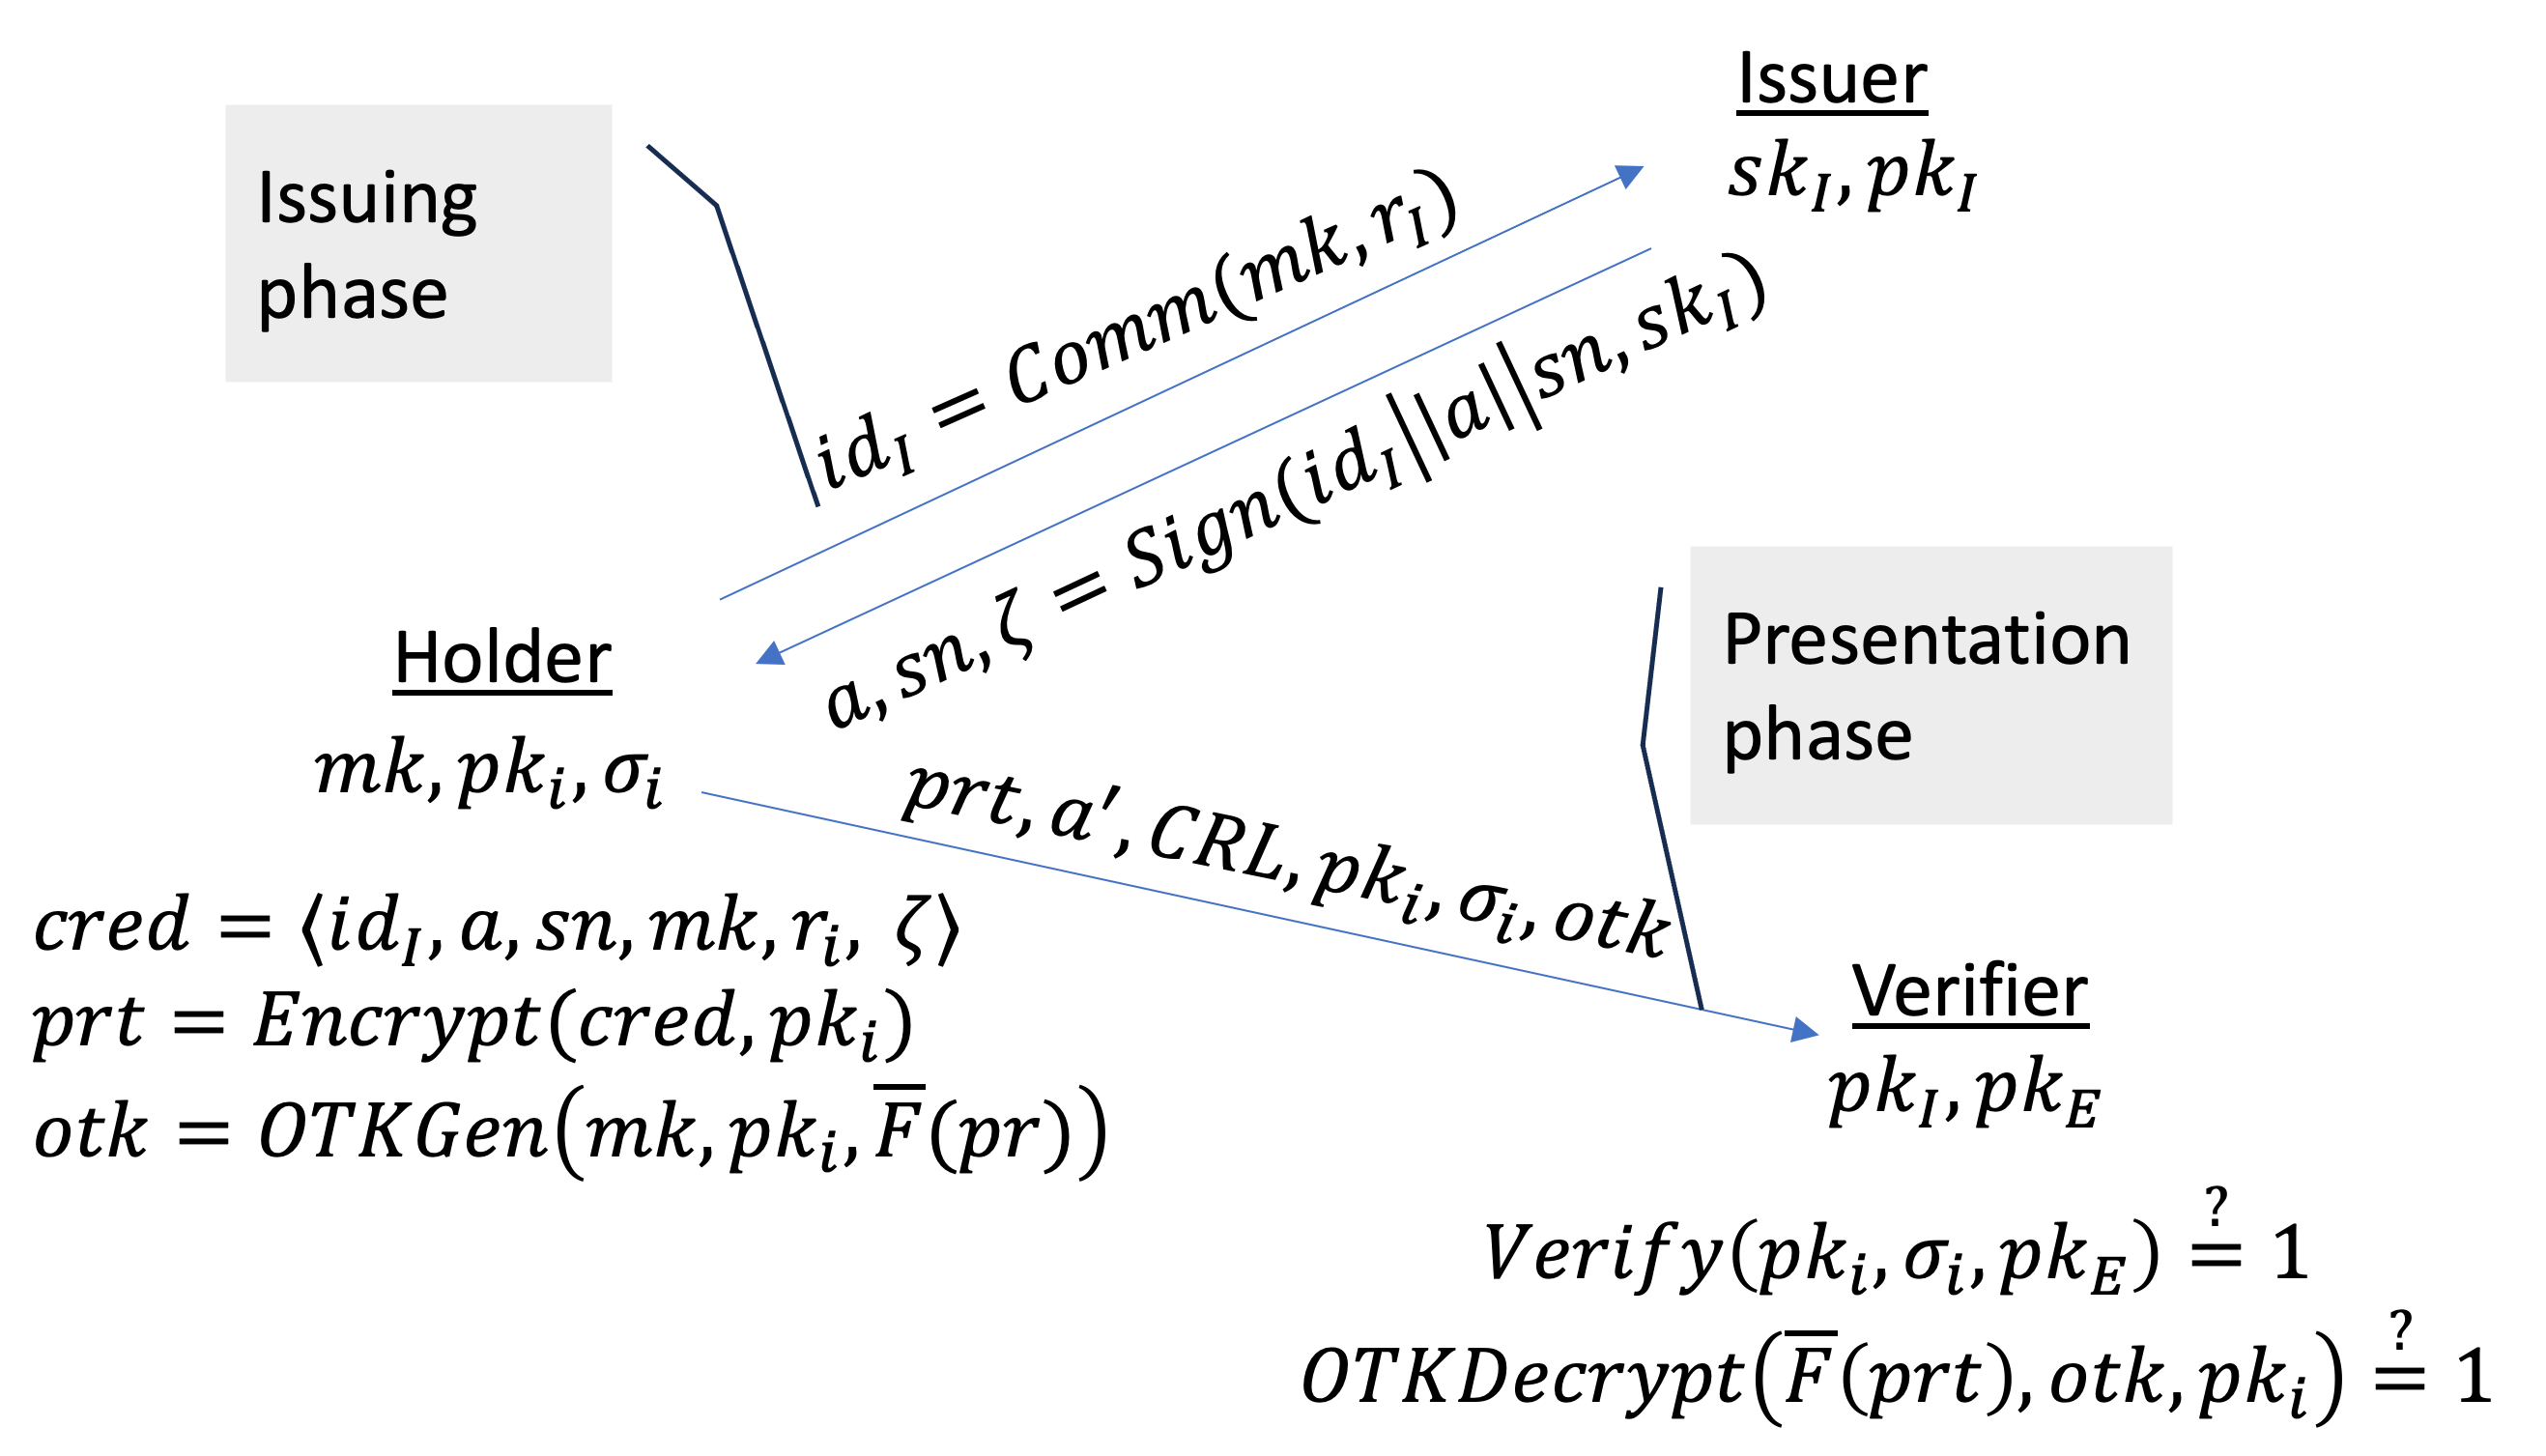
\includegraphics[width=\columnwidth]{schema.png}
\caption{Issuing and presentation phases of the proposed solution.}
\label{fig:schema}
\end{figure}

The issuing phase (cf. Figure \ref{fig:schema}) starts with the holder committing to her secret key ($mk$) while introducing an element of randomness ($r_I$). Subsequently, she uses this commitment $id_I=\bkw{Comm}(mk,r)$ as her unique identifier for a specific issuer $I$. The issuer, in turn, takes the commitment $id_I$, some attributes of the holder $a$ and the serial number $sn$ of the credential, signs all with the issuer's secret key $sk_I$ and returns the signature $\varsigma=\bkw{Sign}(id_I\|a\|sn,sk_I)$, the attributes $a$ and the $sn$ number back to the holder.

In the presentation phase (cf. Figure \ref{fig:schema}), the holder encrypts the credential $cred =\langle id_I, a,  sn, mk, r_i, \varsigma\rangle$, with a homomorphic encryption algorithm and one of her public keys $pk_i$. 

Then, the holder sends the presentation message, with:
\begin{itemize}[noitemsep]
\item The resulting presentation ciphertext $prt = \bkw{Encrypt}(cred,pk_i)$,
\item The holder's attributes to be revealed $a'$ (not necessarily the attributes $a$ in the credential $cred$),
\item The public key $pk_i$ used to encrypt the credential and the correspondent signature from the escrow service $\sigma_i$,
\item A decryption key $otk=\bkw{OTKGen}(mk,pk_i,\overline{F}(prt))$ that can only be used to decrypt a specific homomorphic computation $\overline{F}(prt)$ over the presentation ciphertext $prt$, and
\item A certificate revocation list $CRL$ containing the serial numbers of revoked credentials (which could also be taken from someplace else, e.g. a distributed ledger).
\end{itemize}

The function $\bkw{OTKGen}$ generates a special decryption key $otk$ that allows the delegation of the decryption of a specific ciphertext to the verifier without delegating the decryption of all ciphertext encrypted with the same key. (cf. Section \ref{sec:otk}).

Upon receiving the presentation message, the verifier:
\begin{itemize}[noitemsep]
\item Checks the signature $\sigma_i$ on the public key $pk_i$ of the holder,
\item Recomputes and decrypts $\overline{F}(prt)$, with the $otk$ and the holder's public key,  and checks if the result is valid \[\bkw{OTKDecrypt}(\overline{F}(prt),otk,pk_i)\stackrel{?}{=}1\]
\end{itemize}

The homomorphic computation $\overline{F}(prt)$ that both the holder and the verifier must perform on the encrypted credential $prt$, is the conjunction of four elements $\overline{F}(prt) = prt_{oc} \wedge prt_v \wedge prt_{CRL} \wedge prt_a$, each of them being the result of a specific homomorphic test (see Table \ref{tab:hcomp}).
The first test $prt_{oc}$ checks that the user owns the commitment $id_I$, opening the commitment with the secret key of the holder $mk$ and the randomness $r_I$ used to create the commitment. The second test $prt_v$ checks the signature of the credential with the public key of the issuer $pk_I$. The third test $prt_{CRL}$ checks that the credential serial number is not in the issuer's CRL, and finally the last test $prt_a$ checks that the derived attributes $a'$ are consistent with the signed attributes $a$. The homomorphic test $\overline{Check}$ depends on the specific attributes $a$ and $a'$, for example, if $a$ contains an address with an EU member state and the holder wants to prove that that address is from an EU member state, it can be implemented with the ``Private Set Membership'' primitive $\overline{\bkw{PSM}}(prt,EU)$, which tests that the member state in the address is one of the EU member states, without revealing the member state in the address. 

\begin{table}[ht]
    \renewcommand*{\arraystretch}{1.3}
    \centering
    \begin{tabular}{l|l|l}\hline
         Element & Homo. Test & Result \\\hline
         $prt_{oc}$ & $\overline{\bkw{OpenCom}}(prt)$ & $\senc{\bkw{OpenCom}(id_I,mk,r_I)}{pk_i}$ \\\hline
         $prt_{v}$ & $\overline{\bkw{Verify}}(prt,pk_I)$ & $\senc{\bkw{Verify}(id_I \|a\|sn,\varsigma,pk_I)}{pk_i}$\\\hline
         $prt_{CRL}$ & $\overline{\bkw{PSM}}(prt,CRL)$ & $\senc{sn \notin CRL}{pk_i}$\\\hline
         $prt_a$ & $\overline{Check}(prt,a')$ & $\senc{Check(a,a')}{pk_i}$\\\hline
    \end{tabular}
    \caption{Homomorphic tests performed over the credential presentation.}
    \label{tab:hcomp}
\end{table}

Note that the credential presentation is not traceable by any combination of verifiers and issuers because it is always a fresh encryption and the encrypted values are never revealed to the verifier. 

The following section introduces some background and notation required by the remaining sections, which describe each of the previously used primitives. Section \ref{sec:otk} describes the primitives $\bkw{Encrypt},\bkw{OTKGen}$, and $\bkw{OTKDecrypt}$, while the primitive $\overline{\bkw{PSM}}$ is described in Section \ref{sec:comparison}. Section \ref{sec:owner} describes the primitives $\bkw{Comm}$, $\bkw{OpenCom}$ and $\overline{\bkw{OpenCom}}$, and the primitives $\bkw{Sign}$, $\bkw{Verify}$, and $\overline{\bkw{Verify}}$ are described in Section \ref{sec:sig}.


\section{Background}
\subsection{Notation}

A number is denoted by a lowercase letter, for example, $z \in \Z$. We denote generic sets by a capital letter $S$ and the size of $S$ by $|S|$. The vectors will be written in column form using the arrow notation $\vvv$, where $v_i$ denotes the $i^{th}$ element. The inner product of two vectors is denoted by $\inprod{\vx}{\vy}=\vx^T\vy$. Unless stated otherwise, the norm of a vector $\vvv$ is the $l_2$ norm and is denoted by $\|\vvv\|$. The set of residue classes modulo $q$ is denoted by $\Z_q$, and the class representatives of $\Z_q$ are taken from the half-open interval $[-q/2, q/2)$. 

Let $A \in \Z_q^{n\times m}$, denote 
\[\Lambda^{\perp}_A = \{\vz \in \Z^m :A\vz=\0 \bmod q\}\] as the q-ary lattice of all elements $\vz$ that satisfy the relation $A\vz=\0 \bmod q$. 

A random variable $x$ sampled from a distribution $\D$ is $x \from \D$. 
For a vector $\vvv \in \R^n$, a positive real $s$, and a lattice $\Lambda \subset \R^n$, let $\D_{\Lambda,\vvv,s}$ denote the n-dimensional discrete Gaussian distribution over $\Lambda$, centered at $\vvv$, with parameter $s$. We use $\U_{S}$ to denote a discrete uniform distribution over a set $S$, $\T$ denotes a discrete ternary uniform distribution over $\{-1, 0, 1\}$, and $\chi$ denotes an error distribution $\D_{\Lambda,\0,\sigma}$, with $\sigma$ satisfying the \ac{RLWE} security reduction \cite{lyubashevskyIdealLatticesLearning2010} for the security parameter $\lambda$. The default value $\sigma$ in the HELIB\footnote{\url{https://github.com/homenc/HElib}} and PALISADE\footnote{\url{https://gitlab.com/palisade/palisade-release}} libraries is $\sigma=3.2$.

We will use the following simple lemmas, for which we sketch the proof of the first.
\begin{lemma}\label{lm:binary}
For any odd prime number $p$ and $0\leq x < p$,  $x(x-1)=0 \bmod p$ iff $x=0$ or $x=1$.
\end{lemma}
The proof is straightforward. Since $p$ is prime and $x(x-1)=k.p$ for some $k\in\Z$ then either $x=r.p$ or $x-1=r.p$ for some $r\in \Z$, and because the only $r \in \Z$ satisfying $0\leq x < p$ is $r=0$, then $x=0$ or $x=1$

\begin{lemma}\label{lm:sign}
For any odd prime number $p$ and $-p/2\leq x < p/2$,  $(x+1)(x-1)=0 \bmod p$ iff $x=-1$ or $x=1$ and $x(x+1)(x-1)=0 \bmod p$ iff $x=0, x=-1$ or $x=1$.
\end{lemma}

\subsection{Cyclotomic Rings}

Let $\intring = \Z[X]/\langle \cyclpoly{m} \rangle$ be the cyclotomic ring, isomorphic to the extension field $\Q(\xi_m)$ constructed by adjoining a primitive $m^{th}$ root of unity, where $m$ is a positive integer and $\cyclpoly{m}(X)$ is the $m^{th}$ cyclotomic polynomial, and let $\intring_q=\Z_q[X]/\cyclpoly{m}(X)$ be the module $q$ cyclotomic polynomial. Our implementation uses $\cyclpoly{m}(X) = x^d+1$, with $m=2d$ and $d$ a power of 2. Whenever relevant, we denote the underlying ring with both parameters by $\intring_{d,q}=\Z_q[X]/(x^d+1)$.

We denote by bold lowercase letters the elements of $\pa \in \intring$ and by $\pv{a}$ the vector of elements of $\intring$. The $i^{th}$ element of a vector $\pv{a}$ will be denoted by $\pa_i$ and the $j^{th}$ coefficient of polynomial $\pa$ by $a_j$. Similarly, $a_{i,j}$ will denote the $j^{th}$ coefficient of the $i^{th}$ polynomial of a vector $\pv{a}$. The $l_2$ norm $\|\pv{a}\|$ is defined as $\|\pv{a}\|=\sqrt{\sum a_{i,j}^2}$ and the expansion factor of $\intring$ is defined as $\expfactor = \max{\|\inprod{\pv{a}}{\pv{b}}\|/(\|\pv{a}\|.\|\pv{b}\|) : \pv{a}, \pv{b} \in \intring^k}$. 

Let $n=\eulerphi{m}$ where $\phi$ is Euler’s totient function, and $q > 1$ be a number coprime to $m$, then $\cyclpoly{m}(X)$ splits modulo $q$ into $l_{\Phi}$ irreducible factors of same degree $d$, i.e. $\cyclpoly{m}(X) = \prod_{i=1}^{l_{\Phi}} F_i(X) \bmod q$, where $\delta$ is the order of $q$ modulo $m$, and $l_{\Phi} = n/\delta$. Then by \ac{CRT}, the modulo $q$ cyclotomic polynomial $\intring_q = \Z_q[X]/\cyclpoly{m}(X)$ is congruent with $\intring_q \cong \prod_{i=1}^{l_{\Phi}} \Z_q[X]/\langle F_i(X) \rangle \bmod q$. Each quotient ring $\Z_q[X]/\langle F_i(X) \rangle$ constitutes a \ac{SIMD} slot, isomorphic to the field $\F_{q^{\delta}}$. Therefore, the additions and multiplications of rings in $\intring_q$ result in the corresponding coefficient-wise operations of the respective slots. We denote by $\vv{\sigma}(\pa)$ the canonical embedding vector of the polynomial $\pa$ and by $\sigma(\pa)_i$ the embedded slot $i^{th}$ in the polynomial $\pa$. Let $\pv{a} \in \intring^n_{d,q}$, we denote by $\vv{\sigma}(\pv{a}) = [\vv{\sigma}(\pa_0),\ldots,\vv{\sigma}(\pa_{n-1})]$, the concatenation of the canonical embedding in every polynomial $\pa_i$. 

We will use canonical embedding extensively to pack different attributes into a polynomial, and even to pack smaller polynomials $\pa,\pb \in \intring_{d,q}$ into a larger polynomial $\pc \in \intring_{d',q}$. Assume that $d|d'$ and $q \bmod 2d = 1$ both rings are fully split into $d$ and $d'$  slots, isomorphic to the field $\F_q$. We say that $\pc \in \intring_{d',q}$ embeds the polynomials $\pa,\pb \in \intring_{d,q}$ if $\vv{\sigma}(\pc)=[\vv{0},\vv{\sigma}(\pa),\vv{\sigma}(\pb)]$, where $\vv{0}$ is a padding vector.

\subsection{Hard Problems}

The security of the proposed schema is based on two well-known computational problems, Ring-SIS ($\RSIS$) \cite{peikertEfficientCollisionResistantHashing2006}\cite{lyubashevskyGeneralizedCompactKnapsacks2006} and Ring-LWE (\ac{RLWE}) \cite{lyubashevskyIdealLatticesLearning2010}.

\begin{definition}
($\RSIS_{d,q,m,\beta}$ \cite{langloisWorstcaseAveragecaseReductions2015}) Given $\pv{a}\in\intring_{d,q}^m$ chosen independently of the uniform distribution, with $m\geq \log q$, find $\pv{z}\in\intring_{d,q}^m$ such that $\inprod{a}{z} = 0 \mod q$ and $0<\|\pv{z}\|\leq\beta$. An adversary $\A$ is said to have advantage $\epsilon$ in solving $\RSIS_{d,q,m,\beta}$ if it is able to generate a vector $\pv{z}\in\intring_{d,q}^m$ with norm bounded by $0<\|\pv{z}\|\leq\beta$ such that $\inprod{a}{z} = 0 \mod q$, with a non-negligible probability.
\end{definition}

\begin{definition}
($\RLWE_{d,q,m,\sigma}$ \cite{langloisWorstcaseAveragecaseReductions2015}) Let $\pa,\pb \in \intring_{d,q}$ be two uniformly random polynomials and let $\ps,\pe \in \intring_{d,q}$ be sampled from the Gaussian distribution $\chi$. An adversary $\A$ is said to have an advantage over $\RLWE_{d,q,m,\sigma}$ if it is able to distinguish $(\pa,\pb)$ from $(\pa,\pa.\ps+\pe)$, with a non-negligible probability.
\end{definition}


\subsection{Homomorphic Encryption}

The presented anonymous credential solution is adaptable and can be implemented using two homomorphic encryption schemes: BGV and BFV. These schemes are quite similar, with the primary distinction being how they handle message scaling and error during encryption. Both the $\BGV$ and $\BFV$ schemes are compatible within the framework. The encryption and decryption procedures for both schemes are outlined using the adopted notation to provide a comprehensive overview\footnote{We omit the remaining homomorphic operations because our solution will not impact them.}.

\begin{itemize}[label={--}]
    \item $(\pv{sk},\pv{pk}) \from \bkw{KeyGen}(p, l, 1^\lambda)$: Both schemas take the plaintext module $p$, the multiplication depth $l$ and the security factor $\lambda$ as input for the key generation. In both cases, every element is taken from a ring $\intring_q = \Z_q/\cyclpoly{m}(X)$,  with $m=m(\lambda)$ satisfying the security parameter $\lambda$, and $q=q(l,p,m)$ satisfying the multiplication depth $d$. The secret key $\pv{sk} = [-\ps,\p{1}]^T \in \intring_q^2$ is a vector of polynomials, where $\ps$ is a random polynomial with coefficients in $\T$, and $\p{1}$ is a constant polynomial. The public key $\pv{pk}=[\pa,\pb]^T$ is a pair of polynomials $\pa \from \U_{\intring_q}$ and $\pb=\pa.\ps+\tau.\pe \bmod q$, where $\pe \from \chi$, and 
    $\tau = \begin{cases}
        p & \textrm{if } \BGV\\
        1 & \textrm{if } \BFV
    \end{cases}$
    \item $\pv{c} \from \bkw{Encrypt}(\pv{pk},\ppm)$: The encryption procedure takes the public key $\pv{pk}$ and a polynomial $\ppm \in \intring_p$ encoding the message and outputs a ciphertext $\pv{c} = [\pc_0,\pc_1]^T$ with a pair of polynomials $\pc_0 = \pa.\pu+\tau.\pe_1$ and $\pc_1=\pb.\pu+\tau.\pe_2+\Delta.\ppm$ where $\pu \in \intring_q$ is a polynomial with coefficients taken from $\T$, $\pe_1, \pe_2 \from \chi$ and 
        $\Delta = \begin{cases}
        1 & \textrm{if } \BGV\\
        \floor{q/p} & \textrm{if } \BFV
    \end{cases}$
    \item $\ppm \from \bkw{Decrypt}(\pv{sk},\pv{c})$: The decryption process takes the secret key $\pv{sk}$ and the ciphertext $\pv{c}$ and outputs the message $\ppm \in \intring_p$, $\ppm=\Gamma(\p{\rho})$, with \[\p{\rho}=\inprod{\pv{sk}}{\pv{c}}=\Delta.\ppm+\tau.\p{\partial} \bmod q\] and \[\Gamma(\px) = \begin{cases} \px \bmod p & \textrm{if } \BGV\\ \round{p.\px/q} \bmod p & \textrm{if } \BFV\end{cases}\]
    In both schemas, the decryption algorithm holds if the ciphertext error level $\|\p{\partial}\|_{\infty} < q/2p$.
\end{itemize}
We denote by $\enc{\{x_1,\ldots,x_n\}}$ the encryption of a packed vector $\{x_1,\ldots,x_n\}$ isomorphic to the field $\F^n_{p^\delta}$, with either $\BGV$ or $\BFV$, and by $\enc{\pa}=\enc{\vv{\sigma}(\pa)}$ the encryption of a polynomial $\pa \in \intring_{d,p}$ encoding a cannonical embedding vector $\vv{\sigma}(\pa)$ isomorphic to the field $\F^n_{p^\delta}$. In most cases $p$ and $q$ denote the plaintext and ciphertext modulus of encryption, respectively; however, in some cases, we will encrypt with $\beta.p$ and $\beta.q$, which we denote by $\senc{\pa}{\beta}$. We denote with an overbar $\overline{\bkw{Function}}$ the homomorphic computation of a function with the same name $\bkw{Function}$.

\subsection{Lattice Trapdoors}
In lattice-based encryption, a ``trapdoor'' is a crucial tool that simplifies the solution of complex problems such as LWE or SIS and their counterparts in ring-based cryptography. These problems are inherently difficult without a trapdoor. The key idea behind lattice trapdoors is that LWE and SIS problems become computationally easy when the lattice has bases characterized by short orthogonal vectors, known as "good bases." Conversely, they become computationally hard when the lattice has bases that are not ``good'', referred to as ``bad'' bases"

The ingenious approach involves generating both ``good'' and ``bad'' bases simultaneously. The ``bad'' base is made public, while the ``good'' base is kept confidential as the trapdoor. In many cases, the ``good'' base is a well-known fixed base, and the trapdoor is represented by the unimodular transformation that converts one base into the other. Notably, Micciancio and Peikert's \cite{micciancioTrapdoorsLatticesSimpler2012} solution has been one of the most efficient trapdoor generation methods, demonstrating its effectiveness in solving LWE problems and generating secure solutions for SIS problems.

We are mainly interested in sampling RSIS solutions, that is, finding a polynomial vector $\pv{s} \in \intring_q^{k+2}$, with a short norm such that $\pv{a}.\pv{s}\cong \pc$, for any polynomial $\pc \in \intring_q$. Let
\[\pv{a},\pv{r} \from \bkw{TrapGen}(\lambda)\]
denote the generation of the ``bad'' ($\pv{a}$) and ``good''($\pv{r}$) basis\footnote{$\pv{r}$ is not exactly a good base but one may be generated from it.}, and let
\[\pv{s}\from \bkw{TrapSampl}(\pv{a},\pv{r},\pc)\]
denote the sampling of a polynomial vector $\pv{s}$, such that the Euclidean norm $\|\pv{s}\|<B_t$ is bounded by some parameter $B_t$. The sampling algorithm of \cite{micciancioTrapdoorsLatticesSimpler2012}
requires $q=b^k$ for some $k \in \Z$, which is not always the most appropriate choice of $q$ to be used in $\BGV$ or $\BFV$, since we need $q$ to be as small as possible for efficiency reasons. Also, we use the solution proposed by \cite{cousinsImplementingConjunctionObfuscation2018}. The bound $B_t=\textrm{max } \|\pv{s}\|$ of the Euclidean norm for the preimage samples sampled with this procedure is 
\begin{equation}\label{eq:bound}
    B_t<s\sqrt{d(k+2)}
\end{equation}
where $s=1.3\sigma^2(b+1)(\sqrt{d.k}+\sqrt{2d}+4.7)$ is the spectral bound, and $\sigma=\sqrt{\log_2{2d/\epsilon)}/\pi}$ is the smoothing parameter from which the trapdoor polynomials are generated. 

From \cite{micciancioLatticebasedCryptography2009} we know that the bound $\beta$ that makes $\RSIS_{d,q,m,\beta}$ hard is given by
\begin{equation}\label{eq:rsisbound}
\beta < \textsf{min}(p,2^{\sqrt{4dm\log{q}\log{\delta}}})
\end{equation}
where $\delta$ is the hermite value, which depends on the security parameter $\lambda$. Whenever necessary, we will use $\delta=1.0043$. Therefore, the parameters should be chosen such that $B_t \leq \beta$.

\section{Verifiable Decryption}\label{sec:otk}
A verifiable decryption mechanism is a system that provides an individual with an encrypted value, a way to compute it, and a proof to confirm the accuracy of the decryption process. In this context, the chosen solution, as described in \cite{chillottiHomomorphicLWEBased2016}, involves a one-time self-validating key. This key is used to decrypt a specific encryption as it would be if it was decrypted with the secret key corresponding to a specific public key. However, contrary to the secret key, the one-time key cannot be used to obtain information about any other ciphertext, besides the one for which it was generated.

\begin{definition}
Let $A$ be a set of attributes of a specific user, $V$ be a set of constant values, and a function $m=f(A,V)$. Let $\enc{A}$ be some encryption of $A$ with public key $pk$ and $F(\cdot,\cdot)$ a homomorphic function such that $\enc{m}=F(\enc{A},V)$. A one-time key $k$ for a tuple $(A,V,f,pk)$ is a key of a special algorithm \textsf{OTKDecrypt} that, for $y=F(\enc{A},V)$
\[\textsf{OTKDecrypt}(k,y)= \begin{cases} m & \mbox{if }  \textsf{Valid}(k,y,pk) \\ \perp & \mbox{otherwise} \end{cases}\]
\end{definition} 

\subsection{OTK Encryption Schema} \label{sec:otkschema} 

The proposed solution adheres to the framework presented in \cite{chillottiHomomorphicLWEBased2016} but is tailored to the ring setting with a primary focus on optimizing efficiency. A straightforward approach is to use a \ac{MLWE}-based encryption schema, with a public key matrix $\p{PK}=[\pA,\pv{b}=\pA.\pv{s}+\tau\pv{e}]^T$,  where $\pA,\pR \from \bkw{TrapGen}(\lambda) \in \intring^{k\times 2k+2}_q$, $\pv{s} \from \T^{k.d}$ and $\pv{e} \from \chi^{k.d}$ and a ciphertext
\begin{equation}\label{eq:mcipher}
\enc{\p{m}}=\begin{bmatrix}\pv{c_0}\\\p{c_1}\end{bmatrix}=\begin{bmatrix}\pA.\pv{u}+\tau\pv{e_1}\\\inprod{\pv{b}}{\pv{u}}+\tau\p{e_2}+\Delta.\ppm\end{bmatrix}
\end{equation}


The trapdoor $\pR \in \intring_q^{k\times k+2}$ generated with $\pA \in \intring_q^{k\times k}$, enables the sampling of a polynomial $\pv{x} = \bkw{TrapSampl}(\pA,\pR,\pv{c_0})$ characterized by a small norm, satisfying the equation 
\begin{equation}\label{eq:unvailabletrap}
    \pA.\pv{x}=\pv{c_0}
\end{equation}
where $\pv{c_0} \in \intring^k_q$ is the first element of an encryption $\enc{\p{m}}$ (\cref{eq:mcipher}).

This polynomial $\pv{x}$ can then be used to recover the message $\ppm=\Gamma(\p{c_1}-\inprod{\pv{x}}{\pv{b}} \bmod q)$ without revealing the secret key $\ps$, where $\p{c_1}$ is the second element of the encryption $\enc{\p{m}}$ (\cref{eq:mcipher}).

The polynomial vector $\pv{otk}=\pv{x}$ acts as a decryption key for that specific ciphertext \cite{chillottiHomomorphicLWEBased2016}.
This has the immediate consequence of increasing the dimensionality of the ciphertext, transitioning from $2d$ to $d.(k + 1)$, and the public key, expanding from $2.d$ to $d.k.(k + 1)$. Typically, when transitioning from \ac{RLWE} to \ac{MLWE}, the increase in dimensionality is counterbalanced by a reduction in the ring size. However, in our particular scenario, this adjustment would not only diminish the available data slots but would also exert an influence on the depth of homomorphic multiplications.

Instead, we let the public key be $\pv{pk}=[\pv{a},\pv{b}=\ps\pv{a}+\tau\pv{e}]^T$, where $\pv{a},\pv{r} \from \bkw{TrapGen}(\lambda)$, and let the corresponding ciphertext be
\begin{equation}\label{eq:otkcipher}
\begin{bmatrix}\p{c_0}\\\p{c_1}\end{bmatrix}=\begin{bmatrix}\inprod{\pv{a}}{\pv{u}}+\tau\p{e_1}\\\inprod{\pv{b}}{\pv{u}}+\tau\p{e_2}+\Delta.\ppm\end{bmatrix}
\end{equation}

Then, it is possible to sample $\pv{x} \in \intring_q^{k+2}$ such that $\inprod{\pv{a}}{\pv{x}}=\p{c_0}$, and recover the message $\ppm=\Gamma(\p{c_1}-\inprod{\pv{x}}{\pv{b}})$.
With this approach, the size of the ciphertext does not change, and the public key $\pv{pk}$ increases only by $k+2$, which is much less than with the plain \ac{MLWE} approach.


The polynomial vector $\pv{a}$ generated from the primitive $\bkw{TrapGen}$ has structure $\pv{a} = [1, \p{a_0},\ldots,\p{a_k}]$, where $\p{a_0}$ is a randomly generated polynomial and $\p{a_1}$ to $\p{a_k}$ are statistically indistinguishable from random polynomials. As a result, all except one of the $k + 2$ columns in the public key $\pv{pk}=[\pv{a},\pv{b}=\ps\pv{a}+\tau\pv{e}]^T$ consist of plain \ac{RLWE} samples, $\pv{pk_i}=[\p{a_i}, \ps.\p{a_i}+\tau.\p{e_i}]$, ensuring that they do not reveal information about polynomial error $\p{e_i}$ or secret key $\ps$. However, the first column is represented by $\pv{pk_0}=[1,\ps+\tau\p{e_0}]^T$, which can potentially expose the secret key if the distribution of the secret key is different from the distribution of $\tau.\p{e_i}$. Aligning both distributions resolves this potential issue.
 
The One Time Key schema is similar to the BGV/BFV schema except for the following algorithms:

\begin{itemize}[label={--}]
    \item $(\pv{sk},\pv{pk}, \pv{mk}) \from \bkw{KeyGen}(p, d, 1^\lambda)$: The key generation procedure generates one more key than the BGV/BFV schema: the trapdoor master key $\pv{mk}$, concretely
    \begin{equation*}
    \begin{split}
        \pv{a}, \pv{mk} &\from \textsf{TrapGen}(\lambda)\\
        \pv{sk}&=[-\ps,1]^T\quad \ps \from \chi^n \\
        \pv{pk}&=[\pv{a},\pv{b}]^T\quad \pv{b}=\ps.\pv{a}+\tau.\pv{e} \quad \pv{e} \from \chi^{d(k+2)}\\
    \end{split}
    \end{equation*}
    \item $\pv{c} \from \bkw{Encrypt}(\pv{pk},\p{m})$: The encryption procedure is slower than the original one, given the size of the public key $\pv{pk} \in \intring_q^{2(k+2)}$, but it outputs a ciphertext of the same size $\pv{c}=[\p{c_0},\p{c_1}]^T \in \intring_q^2$ (\cref{eq:otkcipher}), where $\pv{u} \in \intring_q^{k+2}$ is a vector of polynomials with coefficients sampled from $\T$.
    \item $\pv{otk} \from \bkw{OTKGen}(\mathbf{\pv{pk}},\pv{mk},\pv{c})$: The generation of the one-time key $\pv{otk}$ for a ciphertext $\pv{c}$ takes the master key $\pv{mk}$, the public key $\pv{pk}$ and the ciphertext $\pv{c}=[\p{c_0},\p{c_1}]^T$. Thus, a one-time key cannot be built before the computation of the ciphertext, which is not ideal. The $\pv{otk} \in \intring_q^{k+2}$ is sampled from 
    \begin{equation*}
        \pv{otk}=\bkw{TrapSamp}(\pv{a},\pv{mk},\p{c_0})
    \end{equation*}   
    \item $\ppm \from \bkw{OTKDecrypt}(\pv{pk},\pv{otk},\pv{c})$: OTK decryption takes the one-time key $\pv{otk}$, the public key $\pv{pk}=[\pv{a},\pv{b}]^T$ and the ciphertext $\pv{c}=[\p{c_0},\p{c_1}]^T$ as input and outputs the message $\ppm \in \intring_q$ or $\perp$. The algorithm starts by checking that $\|\pv{otk}\| < B$ is less than the maximum bound (vide \cref{eq:bound}), and that $\pc_0-\inprod{\pv{otk}}{\pv{a}}=\pv{0}$ and outputs $\ppm=\Gamma\left(\p{c_1} - \inprod{\pv{otk}}{\pv{b}} \bmod q\right)$, if both conditions hold and $\perp$ otherwise.
\end{itemize}

\subsection{Soundness \& Security} It is easy to see that the OTK decryption algorithm is sound, provided that the public key is of the form $\pv{pk}=[\pv{a},\pv{b}=\ps.\pv{a}+\tau.\pv{e}]$ and the error rate $\partial$ of the ciphertext $\pv{c}$ does not exceed $\partial < q/2p - \delta_{\intring}.n.k.B.B_t$.
\begin{align*}
    \ppm&=\Gamma\left(\p{c_1} - \inprod{\pv{otk}}{\pv{b}} \bmod q\right)
    =\Gamma(\p{c_1} - \inprod{\pv{otk}}{\pv{a}}s+\tau.\inprod{\pv{otk}}{\pv{e}})\\
    &=\Gamma(\p{c_1} - \p{c_0}.s+\tau.\inprod{\pv{otk}}{\pv{e}})
    =\Gamma(\Delta.\ppm+\tau.\p{\partial} + \tau.\inprod{\pv{otk}}{\pv{e}})
\end{align*}
Equality holds if 
\begin{align*}
    &\|\p{\partial} + \inprod{\pv{otk}}{\pv{e}}\|_{\infty} < q/2p \Leftrightarrow
    \|\p{\partial}\|_{\infty} < q/2p + \|\pv{otk}\|_{\infty}.\|\pv{e}\|_{\infty} \\
    &\Leftrightarrow \|\p{\partial}\| < q/2p + s.B
\end{align*}

The security of the resulting schema follows if any pair $(\pv{pk},\pv{c})$ is still indistinguishable from random for any polynomial-time algorithm, as it is the underlying schema, and if the tuple $(\pv{pk},\pv{otk},\pv{c}')$ is indistinguishable from random for any polynomial-time algorithm for any $\pv{c}' \neq \pv{c}$. Both indistinguishability may be proven by hybrid arguments that we sketch below.

The public key $\pv{pk}$ comprises $k+2$ polynomial vectors, $[\pa_i,\pb_i]_{i=0}^{k+2}$, where $\pa_0=1$, $\pa_1=\pa' \from \U_{\intring_q}$ is a uniform random polynomial, and $\pa_j$ for $1<j<k$ are polynomials indinstinguishable from random. Each public key vector $[\pa_i, \pa_i.\ps+\pe_i]$, $i\neq 0$ is also an \ac{RLWE} sample and may be replaced by random instances. The first column of the public key is given by $[1, \ps + \pe_0]$, where $\ps, \pe_0 \from \chi^n$ are two random Gaussian values taken from the same distribution, thus revealing nothing. Finally, by the indistinguishability of the underlying schema, we find that $(\pv{pk},\pv{c})$ is indistinguishable from random for a polynomial-time algorithm with an advantage greater than $\epsilon$.

The same strategy may be followed for the tuple $(\pv{pk},\pv{otk},\pv{c}')$. As before, $\pv{pk}$ may be replaced by a random polynomial vector, as, by construction, $\pv{otk}$ reveals nothing about $\pv{mk}$\cite{micciancioTrapdoorsLatticesSimpler2012}. If it were possible to devise a distinguisher algorithm $\D$ that given $\pv{pk}$ and $\pv{otk}$ was able to distinguish $\pv{c}'=[\pc'_0, \pc'_1]^T$, where $\pc'_0 = \inprod{\pv{a}}{\pv{u}'} + \pe_1$, $\pc'_1 = \inprod{\pv{b}}{\pv{u}'} + \pe_2 + \Delta.\ppm'$, from $\pv{c}''=[\px, \py]^T$, $\px,\py \from \U_{\intring_q}$ then it would be possible to build a distinguisher $\D'$ that given $\pv{pk}$ was able to distinguish $\pv{c}'=[\pc'_0, \pc'_1]^T$ from $\pv{c}''=[\px, \py]^T$, by generating a random $\pv{otk} \from \D_{\Lambda,\pv{0},\sigma}$, creating a ciphertext $\pv{c}=[\inprod{\pv{a}}{\pv{otk}},\pz]$ and feeding $\D$.

\subsection{Efficiency}

Although the key generation and encryption algorithms in the proposed encryption scheme share a structure similar to the underlying BFV schema, they demonstrate reduced efficiency. This efficiency decrease is primarily attributed to a significant increase in the size of the public key, which becomes $k + 2$ times larger. To improve operational efficiency, it is crucial to set the value of $k$ to the smallest feasible value, denoted $k = \ceil{\log_b q}$.

However, this optimization faces limitations due to the "Double CRT" representation constraint, which requires $k$ to satisfy the inequality $k \ge 2l_q+2$. Here, $l_q$ represents the count of pairwise coprime values $q_i$ that make up the modulo $q=\prod_i^l q_i$, restricting the reduction of $k$ beyond a certain threshold.

The proposed solution has been implemented in PALISADE\footnote{\url{https://github.com/ribeirocn/palisade-sfdk}}, and performance results (Table \ref{tab:otk}) confirm that except for ``Key Generation'' and ``Encryption'', other BFV operations do not show a decrease in performance, i.e., $\textrm{SlowDow}=\frac{T_\OTK - T_\BFV}{T_\BFV} = 0$. ``Key Generation'' is $4.9$ times slower due to the construction of the special public key, and ``Encryption'' is $2.3$ times slower, mainly due to the larger size of the public key. The most significant drawback is the generation of $\pv{otk}$, which takes almost $18$ times the elapsed time of a multiplication.



\begin{table}[htbp]
%\setlength\tabcolsep{3pt}
\caption{OTK homomorphic schema performance}
\begin{center}
\begin{tabular}{lr@{\extracolsep{4pt}}rRrr}
\hline
& \multicolumn{2}{c}{$\OTK$ ($\mu s$)} & \multicolumn{2}{c}{$\BFV$ ($\mu s$)} & \multirow{2}{2em}{Slow Down} \\ \cline{2-3} \cline{4-5}
& $T_\OTK$  & $\sigma$	& $T_\BFV$	& $\sigma$	& \\ \hline
KeyGen & 12855 & 90 & 2615 & 26 & 4.9 \\
MultKeyGen & 4776 & 21 & 4794 & 73 & 0 \\
AutomorphKeyGen &	4789 & 36 & 4778 & 46 & 0 \\
Encryption & 7682 & 45 & 3407 & 28 & 2.3 \\
Decryption & 401 & 4 & 398 & 9 & 0 \\
Add	& 59 & 6 & 56 & 4 & 0 \\
AddInPlace & 32 & 3 & 29 & 9 & 0 \\
MultNoRelin & 4133	& 241 & 4144 & 188 & 0 \\
MultRelin & 5456 & 52 & 5692 & 270 & 0 \\
Automorph & 755 & 19 & 760 & 17 & 0 \\
OTKKeyGen & 96569 & 1167 & - & - & - \\			
OTKDecrypt & 616 & 70 & - & - & - \\ \hline
\end{tabular}
\label{tab:otk}
\end{center}
\end{table}

\subsection{Usage}
OTK soundness requires that the holder's public key be of the form $\pv{pk}=[\pv{a},\ps.\pv{a}+\tau.\pv{e}]$ and that the error rate of the encryption is below some bound $\partial$. The former is ensured by having all the public keys of the holder signed by the key escrow service, and the latter can be checked by having the holder provide an OTK to decrypt the multiplication of the freshly encrypted message by an encryption of zero, with a large error, provided by the verifier. The zero encryption error should be such as to emulate the encryption error at level $l-1$, where $l$ is the multiplication level of the function being evaluated. 
If both requirements are met, the holder may generate the encryption of the message in any way (including randomly) provided that the decryption with the secret key $s$ matches the message she wants to prove.

\section{Homomorphic Comparison}\label{sec:comparison}
The primitive $\OTK$ is intended to decrypt the results of homomorphically evaluated functions (HEFs) that involve arithmetic operations, including comparisons such as equalities and inequalities. For example, in scenarios such as determining whether someone is under 18 years of age or comparing the country of residence with each European Union (EU) member state, since EU addresses usually do not explicitly contain ``EU''or any distinguishing indicator, homomorphic comparisons (HC) pose a significant challenge. Bit-wise Homomorphic Encryption (HE) schemes, such as FHEW and TFHE, offer the fastest HC, with comparisons for two n-bit integers done in $\approx170.n$ microseconds\cite{chillottiFasterPackedHomomorphic2017,chillottiTFHEFastFully2020}.

However, when working with word-based encryption schemes (e.g., BGV, BFV, CKKS), HC performance is not as favourable. Efforts have been made to efficiently implement equality ($EQ_S$) and inequality ($LT_S$) operations within these encryption frameworks. 
\begin{align*}
    &LT_S(a,b) = 
    \begin{cases}
      1, & \text{if } a < b; \\
      0, & \text{if } a \ge b, \\
    \end{cases}   
    &&EQ_S(a,b) = 
    \begin{cases}
      1, & \text{if } a = b; \\
      0, & \text{if } a \neq b. \\
    \end{cases}
  \end{align*}
The implementation of the equality function is straightforward using Fermat's Little Theorem to implement the 
\begin{equation}\label{eq:iszero}
    \mathrm{IsZero}(a-b)=EQ_S(a,b)= 1 - (a-b)^{q-1} \bmod q
\end{equation}
function, often used in practice, although its usage can be challenging due to its sequential multiplications, particularly with large modulus values ($q$).

Kim et al. \cite{kimEfficiencyFHEbasedPrivate2016} introduced an optimization technique. When $a,b \in S=\F_{q^d}$ and $d>1$, they use the multiplicative deep-free Frobenius automorphism operation $x \mapsto x^{q}$. This operation reduces the depth of the equality circuit $EQ(a,b) = 1 - (a-b)^{q^{d}-1}$ from $\ceil{d\log_2(q)}$ to $\ceil{\log_2(d)} + \ceil{\log_2(q-1)}$.

Iliashenko and Zucca~\cite{iliashenkoFasterHomomorphicComparison2021} follow the bit comparison strategy, but instead of bits they split the message into digits that they encode in different slots of plaintext. They use a univariate polynomial to interpolate a function that calculates the sign of the difference between two values
Tan et al.~\cite{tanEfficientPrivateComparison2020} went a bit further by embedding each plaintext in a ciphertext slot, encoding different digits of the plaintext into subfields of $\F_{q^d}$ in each slot. They compared each digit and processed the results using a lexicographic circuit.

One common optimization technique is to use SIMD techniques from certain homomorphic schemes such as BGV and BFV. This involves batching several plaintexts into a single ciphertext, allowing multiple comparisons to be performed simultaneously, which is advantageous when dealing with multiple comparisons over a dataset. Both Tan et al. and Iliashenko and Zucca's solutions use this technique to amortize the cost of each individual comparison.

However, in the ``Anonymous Credentials'' use case, only a single comparison is needed to decide access to an information service, and the values to compare often result from previous calculations involving additions and multiplications, which do not align with the digit decomposition in the proposed encoding. Without digit decomposition, a single comparison of a 15-bit number takes significantly longer ($\sim~4~m~38~s$) with the Iliashenko and Zucca solution compared to the proposed solution ($10s$).








\subsection{Private Set Membership}\label{sec:psm}
Our approach also takes advantage of the \ac{SIMD}, but we aim to optimize a single comparison rather than amortizing the cost over several comparisons. Our comparison primitive is called ``Private Set Membership" (PSM). The $\PSM$ primitive takes an encrypted value $x$ and a set of values $S$ and returns an encryption of 1 if $x\in S$ and an encryption of 0 otherwise.
\begin{equation} \label{eq:psm}
\begin{split}
\PSM: &\intring_q^2,\intring_q^r \rightarrow \intring_q^2\\
      &(\enc{x},\pv{s}) \rightarrow \{\enc{0},\enc{1}\}
\end{split}
\end{equation}
$\PSM$ takes two arguments, an encrypted value $\enc{x}$ and a set $S$ of plaintext values, and outputs $\enc{1}$ if $x \in S$, and $\enc{0}$ otherwise. Encryption $\enc{x}$ is a value of the ring $\intring_q^2$, as defined by the encryption schemas BGV or BFV, while the plaintext values $\upsilon=|S|$ in the set $S$ are packed in a vector $\pv{s} \in \intring_q^r$,  such that $r=\ceil{\frac{\upsilon}{l_{\Phi}}}$ where $l_{\Phi}$ is the number of \ac{SIMD} slots of the ring $\intring_q$. The goal of such encoding is to allow parallel comparison of the encrypted value $\enc{x}$ with every slot value of each element $\ps_i \in \intring_q$ of $\pv{s}$.

\begin{algorithm}
\caption{Simplified PSM Algorithm}\label{alg:psm}
\small
\begin{algorithmic}
\Procedure {$\PSM$}{$\enc{x}$, $\overrightarrow{\bm{s}}$}
    \State $d \gets \max{|\ps_i|}$ 
	\State $\encv{\px} \gets \Call{Spread}{\enc{x},d}$\Comment{\small{Copy $x$ to every slot}}
	\State $\encv{\po} \gets \Call{SubProd}{\encv{x}, \overrightarrow{\bm{s}}}$ \Comment{\small{Calculate: $\prod_{i=0}^{r-1} \enc{\p{x}}-\ps_i$}}
	\State $\encv{\po} \gets \Call{IsZero}{\encv{o}}$\Comment{\small{Map every slot to $\enc{0}$ or $\enc{1}$}}
	\State $\enc{\po} \gets \Call{SumAll}{\encv{o},d}$ \Comment{\small{Add all slots}}
    \State \Return $\enc{\po}$
\EndProcedure
\end{algorithmic}
\end{algorithm}

The simplified $\PSM$ algorithm (Algorithm \ref{alg:psm}) has four simple homomorphic steps. The first step copies the encrypted value $\enc{x}$ in the first slot into all other $l_{\Phi}-1$ slots. The result is an encryption of a packed vector $\enc{\px} = \enc{\{x,\dots,x\}} \in \intring_q$ with $l_{\Phi}$ copies of $x$. The second step executes a \ac{SIMD} subtraction of $\enc{\px}$ from every element of $\pv{s}$ and calculates the \ac{SIMD} product of the result $\enc{\po} = \prod_{i=0}^r (\enc{\px}-\ps_i) \bmod q$. The result $\enc{\po} \in \intring_q^2$ is a packed encryption of a vector $\vo$, with at most one zero element, the one that matches the searched value. Notice that the last element of the vector $\pv{s}$ may not have all slots filled, thus requiring padding, which is done by ciphertext stealing the result of the previous product. The third step computes the $\mathrm{IsZero}(a)$ (\cref{eq:iszero}) function on every slot at the same time. Finally, the fourth step adds all the slots and returns the result. In general, the algorithm computes the function $\PSM(x,s)$ homomorphically (\cref{eq:psmimp}),
taking advantage of the \ac{SIMD} techniques as much as possible.
\begin{equation}\label{eq:psmimp}
    \PSM(x,\pv{s}) =\sum_{j=0}^{l-1} 1-\left(\prod_i^r (x-s_{i,j})\right)
\end{equation}

The third step is the most expensive since it requires $\log(q-1)$ multiplications to calculate the exponentiation by iterative squaring. The first step is computed using an algorithm similar to iterative squaring, but instead of squaring the result at each iteration, it uses the automorphisms of the ring setting $\intring_q$ to rotate and add $\log(l_{\Phi})$ times (Appendix \ref{app:psmalgorithms}). The second step requires $r-1$ multiplications. However, for large ring dimensions, the number of available slots $l$ is often larger than $|S|$, so $r=\ceil{|S|/l}=1$ and no multiplications are required. The last step also does not require multiplications. It adds all the slots and leaves the result in the first slot. It follows a strategy similar to the \textsc{Spread} function, but in the reverse direction (Appendix \ref{app:psmalgorithms}). As such, it also requires $\log(l_{\Phi})$ rotations and additions.


\subsection{Applications and Performance}

Within the ``Anonymous Credential" setting, the $\PSM$ primitive can be used to check the following:
\begin{itemize}
\item if an address is within the EU, by checking if the name of the country in the address is one of the member states without revealing the address;
\item if the OID of the credential is listed in a CRL without revealing the OID;
\item if someone is under 18 years old at a specific date without revealing her age;
\item if some encrypted value is less than another encrypted value.
\end{itemize}
However, the usage strategies differ. The most straightforward is to check the OID of the credential. It only requires packing the CRL list in the vector $\Vec{s}$ and running $\PSM(\enc{oid},\Vec{s})$. For some RLWE settings, it is possible to pack in $\Vec{s}$ more than 100K OIDs at the cost of only 2 or 3 additional multiplications (second step of algorithm \ref{alg:psm}).

\subsubsection{Integer Comparison}
Checking if someone is under 18 years of age or if an encrypted value $a$ is less than another encrypted value $b$ follows a similar strategy. We compute the difference between both values $a-b$ or between the birthdate and the current date and check if the result is in a specific set. If the result is in a set with all possible negative values ($\F_q^{-}=[-(q-1)/2,-1]$), or with all possible ages (in days) between $0$ and $18$ years ($S=\{0,\ldots,\sim6570\}$) then $a<b$, or someone is under 18.

Iliashenko and Zucca \cite{iliashenkoFasterHomomorphicComparison2021} made available an implementation of their solution\footnote{https://github.com/iliailia/comparison-circuit-over-fq}. For comparison purposes, we have extended their implementation with our one\footnote{https://github.com/ribeirocn/comparison-circuit-over-fq} and tested both in the conditions required by the current setting:
\begin{itemize}
    \item Just one comparison, thus time is not amortised over multiple comparisons;
    \item No digit decomposition, thus each value is contained in a single slot, and each slot may contain a single number in $\F^{+}_q$.
\end{itemize}
Table \ref{tab:integer} contains the parameters chosen for various domain sizes with a logarithmic scale $\log_2{|S|}$, for both the PSM and the univariate schemas of \cite{iliashenkoFasterHomomorphicComparison2021}. 

\begin{table}[htbp]
\setlength\tabcolsep{3pt}
\caption{Integer Comparison Settings}
\begin{center}
\begin{tabular}{cccccccc}
\hline
$\log_2{|S|}$ & p & m & $l_{\Phi}$ & $\lambda$ & $\log_2{q}$ & Univ & PSM \\ \hline
6 & 131 & 25743 & 4290 & 161 & 260 & 4.08 s & 2.75 s\\ 
9 & 1031 & 24247 & 898 & 145 & 400 & 13.29 s & 4.62 s \\
10 & 2053 & 35443 & 1518 & 189$^\mathrm{a}$ & 450$^\mathrm{b}$ & 30.75 s & 8.97 s\\
12 & 8209 & 39283 & 6480 & 171$^\mathrm{c}$ & 560$^\mathrm{d}$ & 77.56 s & 13.00 s\\
15 & 65537 & 65536 & 32768 & 104 & 730 & 256.50 s & 9.59 s\\
\hline
\multicolumn{8}{l}{$^\mathrm{a,b,c,d}$ differ slightly in PSM version: $^{\mathrm{a}}$193, $^{\mathrm{b}}$440, $^{\mathrm{c}}$175, $^{\mathrm{d}}$550.}
\end{tabular}
\label{tab:integer}
\end{center}
\end{table}

We have run experiments with message bit sizes of 6 to 15. For sizes above 15 bits, the time spent initializing the cryptography context is too large. The 15-bit setting is itself a particular case. Given that the order $d$ of $q$ modulo $m$ is 1, the number of available slots $l_{\Phi}=n/d$ is given by the size of the ring $n=|\intring_q|=\eulerphi{m}$. Such a large $l_{\Phi}$ simplifies the comparison greatly. In particular, all negative values $\F_q^{-}$ fit into a single vector $\vs$ and may be compared simultaneously.

From the results depicted in Fig. \ref{fig:integer}, we may conclude that, for this specific purpose, the PSM solution is always faster than the univariate solution, which was expected from the number of multiplications that both need to perform. For the specific setting, the number of multiplications performed by the Univariate schema is 
\[U(p) \sim \sqrt{2p-4}+3(\log_2{2p-4})/2 + 2\]
while the number of multiplications in PSM is
\[P(p)= (p-1)/2l_{\Phi} + \log_2{p-1}\]
It is easy to show that $U(p)>P(p)$ for any $l_{\Phi}>0$ and $p>2$.

\begin{figure*}[htbp]
\begin{subfigure}{.33\textwidth}
\centering
\begin{tikzpicture}[scale=0.70]
\begin{axis}[
    xlabel={Plain Text Bit Sizes ($\log_2{|S|}$)},
    ylabel={Time [s]},
    xmin=6, xmax=16,
    ymin=0, ymax=260,
    xtick={2,4,6,8,10,12,14,16},
    ytick={0,40,80,120,160,200,240},
    legend pos=north west,
    ymajorgrids=true,
    grid style=dashed,
]

\addplot[
    color=blue,
    mark=square,
    ]
    coordinates {
        (6,2.74577)(9,4.6201)(10,8.97098)(12,12.9959)(15,9.59417)
    };

\addplot[
    color=red,
    mark=*,
    ]
    coordinates {
    (6,4.07774)(9,13.2915)(10,30.7507)(12,77.5586)(15,256.502)
    };
    
\legend{PSM , Univariate}
    
\end{axis}
\end{tikzpicture}
\caption{Efficiency of Integer Comparison.}
\label{fig:integer}
\end{subfigure}
\begin{subfigure}{.33\textwidth}
\centering
\begin{tikzpicture}[scale=0.7]
\begin{axis}[
    xlabel={Plain Text Size (bits)($\log_2{p}$)},
    ylabel={Time [s]},
    xmin=8, xmax=16,
    ymin=0, ymax=65,
    xtick={2,4,6,8,10,12,14,16},
    ytick={0,20,40,60},
    legend pos=north west,
    ymajorgrids=true,
    grid style=dashed,
]

\addplot[
    color=blue,
    mark=square,
    ]
    coordinates {
        (8,24.954)(9,28.7115)(10,22.2222)(16,64.215)
    };

\addplot[
    color=red,
    mark=*,
    ]
    coordinates {
    (8,21.7776)(9,17.4891)(10,14.0714)(16,55.2358)
    };
\legend{Uni Slot, Multi Slot}
    
\end{axis}
\end{tikzpicture}
\caption{PSM efficiency with plaintext size.}
\label{fig:string}
\end{subfigure}
\begin{subfigure}{.33\textwidth}
\centering
\begin{tikzpicture}[scale=0.7]
\begin{loglogaxis}[
    xlabel={Number of strings to search},
    ylabel={Time [s]},
    xmin=10, xmax=6000,
    ymin=30, ymax=310,
    log ticks with fixed point,
    xtick={10,50,250,500,1500,6000},
    ytick={50,75,150,300},
    legend pos=north west,
    ymajorgrids=true,
    grid style=dashed,
]

\addplot[
    color=blue,
    mark=square,
    ]
    coordinates {
        (10,53.42)(50,61)(250,75.4)(500,76.81)(1500,84.97)(3000,85)(6000,86.69)
    };

\addplot[
    color=red,
    mark=*,
    ]
    coordinates {
    (10,34.45)(50,40.16)(250,51.39)(500,55.06)(1500,100.29)(3000,166.41)(6000,309.51)
    };

\legend{Uni Slot, Multi Slot}
    
\end{loglogaxis}
\draw [red,dashed] (4.3,0) -- (4.3,5.75);
\draw [blue,dashed] (6.2,0) -- (6.2,5.75);
\end{tikzpicture}
\caption{PSM efficiency with set size.}
\label{fig:searchspace}
\end{subfigure}
\caption{PSM efficiency}
\end{figure*}

\subsubsection{String Comparison}
$\PSM$ handles string comparison in two ways, resulting from different packaging strategies. Both strategies require minor changes to the $\PSM$ algorithm. The first strategy, called MultiSlot, is to pack each string of size $e$ over $e$ plaintext slots, thus setting the number of strings encoded in each plaintext at most $b=\floor{l_{\Phi}/e}$. The second strategy, dubbed UniSlot, is more compact, but slightly less efficient. It takes advantage of the plaintext ring structure $\F_{p^{\delta}}$, where $\delta$ is the order of $p$ modulo $m$. When $\delta>1$, it is possible to pack several characters in a single slot.

The first strategy requires changing the function {\sc SumAll} because the slots containing the result of the slot-wise comparison of the string with each copy of the pattern must first be multiplied by each other and then only added together, thus requiring additional $\log_2{e}$ multiplications. The second strategy requires changing the {\sc IsZero} function to implement Fermat's Little Theorem on extension fields.
\begin{equation}\label{eq:iszero+}
    \mathrm{IsZero}(a) = 1 - a^{p^{\delta-1}} \bmod p
\end{equation}
Kim et al. \cite{kimEfficiencyFHEbasedPrivate2016} showed that this equation could be implemented with a multiplicative depth of $\ceil{\log_2{\delta}}+\ceil{\log_2{p-1}}$ by taking advantage of the homomorphic Frobenius automorphism $x \mapsto x^{p}$. Therefore, when $\delta=e$, the multiplicative depth of both methods is equal. However, this second strategy also requires $\delta-2$ automorphisms that do not consume depth but do consume time.

Both alternatives impose limits on the search space. The UniSlot strategy forces the size of the pattern string to be no larger than $p^{\delta}$ bits, while the MultiSlot strategy imposes a soft limit on the search space $|S|$. The limit of the UniSlot strategy may be eliminated by combining both strategies, thus packing each string in $e.\delta$ slots. To eliminate the limit of the MultiSlot strategy, the {\sc SubProd} call in Alg. \ref{alg:psm}, must be replaced by a call to a more complex {\sc SubMapAdd} function (Appendix \ref{app:psmalgorithms}).


Tab. \ref{tab:string} compares both strategies for different plaintext modulus $p$. The maximum string size $\nu$ in bytes is set to $\nu=d.\floor{\log_2{p}}/8$ for the UniSlot strategy and $\nu=e.\floor{\log_2{p}}/8$, with $e=16$, for the MultiSlot strategy. The biggest difference between the two approaches is the number of strings that may be compared simultaneously. The UniSlot strategy can, on average, compare ten times more strings simultaneously ($ss_{max}$). 

Regarding efficiency, the UniSlot version is slightly less efficient (Fig. \ref{fig:string}) due to additional $d-2$ automorphisms.

\begin{table}[htbp]
\setlength\tabcolsep{3pt}
\caption{String Equality Settings}
\begin{center}
\begin{tabular}{ccccccccc}
\hline
\multirow{2}{1em}{p} &  \multirow{2}{1em}{$\lambda$} &  \multicolumn{3}{c}{UniSlot} & & \multicolumn{3}{c}{MultiSlot} \\ \cline{3-5} \cline{7-9}
&& $\nu$ & $ss$ & T(s) & & $\nu$ & $ss$ & T(s) \\ \hline
257 &  163 &  21 & 1448 & 24.95 & & 16 & 90 & 21.78\\
521 &  141$^{\mathrm{a}}$&  24 & 1560 & 28.71 & & 18 & 159 & 17.49 \\
1031 &  133 &  21 & 1904 & 22.22 & & 20 & 119 & 14.07 \\
65537 &  164$^{\mathrm{b}}$ &  36 & 3480 & 64.22 & & 32 & 504 & 55.24 \\
\hline
\multicolumn{9}{l}{$^\mathrm{a,b}$ differ slightly in MultiSlot version: $^{\mathrm{a}}$135, $^{\mathrm{b}}$122.}
\end{tabular}
\label{tab:string}
\end{center}
\end{table}


\begin{comment}
\begin{figure}[htbp]

\centering
\begin{tikzpicture}[scale=0.7]
\begin{axis}[
    xlabel={Plain Text Size (bits)($\log_2{p}$)},
    ylabel={Time [s]},
    xmin=8, xmax=16,
    ymin=0, ymax=65,
    xtick={2,4,6,8,10,12,14,16},
    ytick={0,20,40,60},
    legend pos=north west,
    ymajorgrids=true,
    grid style=dashed,
]

\addplot[
    color=blue,
    mark=square,
    ]
    coordinates {
        (8,24.954)(9,28.7115)(10,22.2222)(16,64.215)
    };

\addplot[
    color=red,
    mark=*,
    ]
    coordinates {
    (8,21.7776)(9,17.4891)(10,14.0714)(16,55.2358)
    };
\legend{Uni Slot, Multi Slot}
    
\end{axis}
\end{tikzpicture}
\caption{PSM efficiency with plaintext size.}
\label{fig:string}
\end{figure}
\end{comment}

However, if the search space $|S|>ss_{max}$, then {\sc MultiSlot} is much less efficient due to the {\sc SubMapAdd} algorithm. Fig. \ref{fig:searchspace} depicts the time required to search for different set sizes $|S|$, for 16 character UTF-16 strings (last line of Tab. \ref{tab:string}). Notice that the slope of the {\sc MultiSlot} curve increases when the set to search is larger than $ss_{max}=504$, but that does not happen with {\sc UniSlot} when the search set is larger than $ss_{max}=3480$.

\begin{comment}
\begin{figure}[htbp]
\centering
\begin{tikzpicture}[scale=0.7]
\begin{loglogaxis}[
    xlabel={Number of strings to search},
    ylabel={Time [s]},
    xmin=10, xmax=6000,
    ymin=30, ymax=310,
    log ticks with fixed point,
    xtick={10,50,250,500,1500,6000},
    ytick={50,75,150,300},
    legend pos=north west,
    ymajorgrids=true,
    grid style=dashed,
]

\addplot[
    color=blue,
    mark=square,
    ]
    coordinates {
        (10,53.42)(50,61)(250,75.4)(500,76.81)(1500,84.97)(3000,85)(6000,86.69)
    };

\addplot[
    color=red,
    mark=*,
    ]
    coordinates {
    (10,34.45)(50,40.16)(250,51.39)(500,55.06)(1500,100.29)(3000,166.41)(6000,309.51)
    };

\legend{Uni Slot, Multi Slot}
    
\end{loglogaxis}
\draw [red,dashed] (4.3,0) -- (4.3,5.75);
\draw [blue,dashed] (6.2,0) -- (6.2,5.75);
\end{tikzpicture}
\caption{MultiSlot vs UniSlot PSM efficiency with set size.}
\label{fig:searchspace}
\end{figure}
\end{comment}

\section{Proof of ownership}\label{sec:owner}
The proof of ownership of a credential is no different from the proof of any other attribute. The holder provides the issuer with a committed value, and the issuer includes it as any other attribute. To prove ownership, the holder opens the commitment but does it homomorphically, not revealing the opener or the commitment.

The commitment can be any commitment with a linear opening, such as, for instance, the Ajtai commitment \cite{ajtaiGeneratingHardInstances1996} adapted to the ring setting. In such a commitment scheme, one commits to a secret vector $\pv{s} \in \intring_{d,p}^l$ with a randomness $\pv{r} \in \intring_{d,p}^l$, where both $\|\pv{s}\|$ and $\|\pv{r}\|$ are small, for some public random values $\pv{a}\from \intring_{d,p}^l$ and $\pv{b}\from \intring_{d,p}^l$, by computing the commitment
\begin{equation}\label{eq:commit}
\begin{aligned}
    \bkw{Comm}(&\pv{s},\pv{r})\colon \intring_{d,p}^{2l} \to \intring_{d,p}\\
    &\inprod{\pv{a}}{\pv{s}}+\inprod{\pv{b}}{\pv{r}} \mapsto  \pc
\end{aligned} 
\end{equation}
and sending it to the issuer to be signed, together with the issuers' attributes (cf. section \ref{sec:solution}).

Opening the Ajtai commitment is a matter of revealing the committed value $\pv{s}$ and the randomness $\pv{r}$, and check 
\begin{subequations}\label{eq:commitopen}
\begin{align}
    \bkw{OpenCom}(&\pc,\pv{s},\pv{r})\colon \intring_{d,p}^{2l+1} \to \{0,1\} \nonumber\\
    &\inprod{\pv{a}}{\pv{s}}+\inprod{\pv{b}}{\pv{r}} \stackrel{?}{=} \pc \label{eq:commitopen_a}\\
    &\|\pv{s}\| \textrm{ and } \|\pv{r}\| \textrm{ are small} \label{eq:commitopen_b}
\end{align} 
\end{subequations}
Implementing the commitment opening homomorphically over the presentation ciphertext $\p{prt} = \enc{\p{m}} \in \intring_q$
\begin{equation}\label{eq:hcommitopen}
    \overline{\bkw{OpenCom}}(\p{prt})\colon \intring_{q} \to \enc{\{0,1\}}\\
\end{equation}
can be done efficiently if the presentation $\p{prt}$ is the encryption of the canonical embedding of the different elements of the presentation 
\begin{equation}\label{eq:presentation}
    \p{prt}=\enc{\{\vv{0},sn,\vv{\sigma}(\pc),\vv{\mu},\vv{\sigma}(\pv{\varsigma}),\vv{\sigma}(\pv{o})\}}
\end{equation}
where $\pc$ is the commitment, $\vv{\mu}=\{\mu_0,\ldots\mu_p\}$ is the set of attributes, $\pv{\varsigma}$ is the credential signature (cf. section \ref{sec:sig}), $sn$ is the credential serial number, and $\pv{o}=(\pv{s},\pv{r}) \in \intring_{d,p}^{2l}$ is the commitment opener. Using standard automorphism operations available in $\BGV$ and $\BFV$, the verifier can 
verifier extract $\enc{\pv{s}}$, $\enc{\pv{r}}$ and $\enc{\pc}$ from the presentation $\p{prt} =\enc{\p{m}}$ and verify  homomorphically \cref{eq:commitopen_a,eq:commitopen_b}.

The \cref{eq:commitopen_a} can be checked efficiently homomorphically by computing 
\begin{equation}\label{eq:commitverify}
\SUM_{2l,d}\left((\pv{a},\pv{b}) \odot  \enc{\pv{o}}\right) \ominus \enc{\pc} 
\end{equation}
The result will be an encryption of 0 if the commitment was correctly opened or something else otherwise.
The operators $\odot$ and $\ominus$ denote the element-wise homomorphic multiplication and subtraction, respectively, and $\SUM_{m, n}(\enc{\pv{a}})$ is a homomorphic function that takes $m$ groups of $n$ slots of each encrypted polynomial $\enc{\pa_k}$ and returns an encrypted polynomial $\enc{\pb_k}$ with the first $n$ slots having the group-wise homomorphic addition, and the remaining slots having zero (vide \cref{eq:sumslots}).
\begin{equation}\label{eq:sumslots}
\begin{aligned}
    &\enc{\pv{b}} = \SUM_{m, n}(\enc{\pv{a}})\\
    &\vv{\sigma}(\pb_k)_i  = 
    \begin{cases}
        \overline{\sum}_{j=0}^{m-1} \vv{\sigma}(\pa_k)_{i+j.n} & \text{if } 0\leq i < n\\
        0 & \text{otherwise}
    \end{cases}
\end{aligned}    
\end{equation}
With this approach, checking \cref{eq:commitopen_a} requires only one homomorphic multiplication, $1+\log m$ additions, and $\log m$ automorphisms.

To simplify the process of verifying \cref{eq:commitopen_b}, we restrict $\pv{s}$ and $\pv{r}$ to have $\|\vv{\sigma}(\pv{s})\|_{\infty}=\|\vv{\sigma}(\pv{r})\|_{\infty}=1$, by chosen two random vectors $\vv{s},\vv{r}\from \{-1,0,1\}^{l.d}$ and canonical embedding them in $\pv{s}$ and $\pv{r}$, respectively. The verifier leverages the lemma \ref{lm:sign} to check that every slot of the opener $\vv{\sigma}(\p{o})_i \in \{-1,0,1\}$, and
the norm inequalities\cite{damgardMultipartyComputationSomewhat2012} to ensure that the norm
\[\|\pv{o}\|\leq\sqrt{d.(l+1)}\|\p{o}\|_{\infty}\leq\sqrt{d.(l+1)}\|\vv{\sigma}(\p{o})\|_{\infty}\leq\sqrt{d.(l+1)}\]

The commitment is statistically hiding and computationally binding, provided that $RSIS_{d,p,l,d(l+1)}$ is hard. From \cref{eq:rsisbound} we must set $d,l\geq\log p$ and $p$ so that the bound 
\[B=\sqrt{d.(l+1)}<\textsf{min}(p,2^{\sqrt{4d(l+1)\log{p}\log{\delta}}})\]

For reasons that will be evident in the next section, the plaintext modulus $p$ can be set to a prime number $p\approx O(2^{16})$. Setting $l$ to the minimum admissible value $l=16$, we have $d\ge 1$ for a hermit value $\delta=1.0043$. Choosing $d=4$ ensures a large enough commitment ($2^{64}$) that is not easily guessable. Therefore, the commitment takes only four slots in the credential, and the opening $2.4.16=128$ slots in the encrypted presentation message $\enc{\vv{\sigma}(m)}$. 

As usual, the commitment $\pc$ is the holder's identifier on the issuer. The holder may be known by different commitments $\pc'=\inprod{\pv{a}}{\pv{s}}+\inprod{\pv{b}}{\pv{r}'}$ to the same secret $\pv{s}$, in different issuers, by using different randomizations $\pv{r}'$. In this context, proving the ownership of two credentials from different issuers requires only extending the opener $\pv{o}=(\pv{s},\pv{r},\pv{r}')$ to include both randomizations.


\section{Homomorphic Verification of Encrypted Signatures}\label{sec:sig}
In an ``Anonymous Credentials'' setting, the credential holders should be able to present the same credential several times to the same verifier or different verifiers without revealing their identity or being traced. However, signatures are often immutable to prevent existential forgery attacks, and therefore easily traceable. The classical solution is to replace the signature with a new, fresh zero-knowledge proof that the holder knows the signature for the credential. However, quantum-resistant zero-knowledge solutions in quantum-resistant encrypted data, signed with quantum-resistant signatures, have some challenges\cite{bootleFrameworkPracticalAnonymous2023}. Another approach is to encrypt the signature with a fresh new encryption each time a credential is presented. However, verifying an encrypted signature over encrypted data poses several challenges, with the primary one being the need for homomorphic computability in the verification process.

A signature solution proposed by Lyubashevki et al.\cite{lyubashevskyShorterLatticeBasedGroup2021} could potentially be used. However, it requires a large modulus ($q = O(2^{64})$), which is suboptimal for encryption. When the plaintext modulus is of order $O(2^{64})$, the ciphertext modulus must be of the order $O(2^{128})$, which is impractical for efficient encryption operations.

In the following subsection, we start by proposing a simple GPV-like signature
\footnote{The signature is straightforward and we are not sure that it has never been proposed before, but we could not find it.},
which is not as efficient as most existing lattice-based signatures but fits our homomorphic needs.
Then we show how to implement the signature verification step homomorphically.

\subsection{GPV-like Signature}
The proposed schema is similar to the GPV schema \cite{gentryTrapdoorsHardLattices2008}, but the hash function is replaced by a collision-resistant lattice base hash function and a pseudorandom number generator. The GPV schema uses a trapdoor $\pv{r} \in \intring_p^k$ for a vector $\pv{a} \in \intring_p^{k+2}$
to sample a short vector $\pv{s}$ from a discrete Gaussian in a lattice $\Lambda^{\perp}_{H(\boldsymbol{\mu})}(\pv{a})$,
such that $\inprod{\pv{a}}{\pv{s}}=H(\boldsymbol{\mu}) \bmod p$, where $H:\intring_q \to \intring_q$ is a polynomial hash function.

The proposed schema also samples a short vector $\pv{s}$ from a discrete Gaussian such that
\[\inprod{\pv{a}}{\pv{s}}=\inprod{\pv{b}}{\pv{\mu}}+\pvv_i \bmod p\]
where $\pvv_i$ is the $i^{th}$ element of a pseudorandom number generator $\PRGN(seed)= [\pvv_1,\ldots,\pvv_N] \in \intring_q^{N}$ and $\pv{\mu}\in\intring_p^m$ is a short vector with signed data.

\subsubsection{Signature Definition}
\begin{description}
\item[$\bkw{ParamGen}(1^{\lambda}) \to d,q,m,b,\sigma:$] Generates the schema parameters $(d,q,m,b,\sigma) \in\Z^5$ for the specified security $\lambda$. 
\item[$\bkw{KeyGen}(d,q,m,b) \to \pv{pk},\pv{sk}:$] The key generation phase starts by generating an MP12 trapdoor $(\pv{a},\pv{r}) \from \TrapGen(d,q,b,\sigma)$, with $k=\ceil{\log_b q}$, and $d$ as the ring size. Then it samples $\pv{b}\from \intring_q^m$ and $seed \from \Z$ uniformly. It returns $\pv{sk}=\pv{r} \in \intring_q^k$ and $\pv{pk}=(\pv{a},\pv{b},seed) \in \intring_q^{k+2}\times\intring_q^m\times\Z$
\item[$\bkw{Sign}(\pv{\mu}, \pv{sk}, \pv{pk}) \to \pv{\varsigma}:$] The signature phase starts by checking that $\pv{\mu} \in \intring_q^m$ and $\|\pv{\mu}\|<\sigma_{\mu}$. It gets a one-time public key $\pvv_i \from \PRGN(seed)$, increments i, computes
the syndrome $\pc=\inprod{\pv{b}}{\pv{\mu}}+\pvv_i$, and samples a short vector $\pv{s}=\SamplePre(\pc,\pv{a},\pv{r})$. It returns $\pv{\varsigma} \from (\pv{s},\pvv_i)$
\item[$\bkw{Verify}(\pv{\mu},\pv{\varsigma},\pv{pk}) \to \{1,0\}:$] The signature verification phase checks that 
\begin{align}
    &\inprod{\pv{a}}{\pv{s}}=\inprod{\pv{b}}{\pv{\mu}}+\pvv_i \bmod p \label{eq:ver_a}\\
    &\|\pv{s}\|<B_t \label{eq:ver_b}\\
    &\|\pv{\mu}\|<B_{\mu} \label{eq:ver_c}\\
    &\pvv_i \in \PRGN(seed) \label{eq:ver_d}
\end{align} 

Outputs $1$ if all equations hold and $0$ otherwise.
\end{description}

\subsubsection{Soundness and Security}
The signature schema is trivially correct by the definition of $\bkw{TrapGen}$ since every signature generated by the signing procedure is verified by the verification procedure. 

To prove security, we show that, if there is an adversary $\A$ that can generate a new valid signature $(\pv{\mu},\pv{\varsigma})$ in an existential forgery game, we can build a simulator $\B$ that solves $\RSIS_{d,q,k+2,B_t}$, $\RSIS_{d,q,m,B_{\mu}}$ or $\RSIS_{d,q,m+k+2,\sqrt{B_{\mu}^2+B_t^2}}$ with nonnegligible probability (cf. Appendix \ref{app:sigproof}).
\subsubsection{Parameter Setting}

Setting the signature parameters such that the signature is secure and yet easily encryptable is a challenge. Encrypting polynomials with large plaintext is not efficient; therefore, we choose $p$ to be the smallest possible prime value that is still secure. From \cref{eq:bound} we know that the bound $B_t=\|\pv{s}\|$ on the trapdoor-generated vector $\pv{s}\in \intring_{d,p}^{k+2}$, with $k=\ceil{\log_b{p}}$, is given by
\begin{equation}\label{eq:sbound}
B_t = s\sqrt{d(k+2)}   
\end{equation}
and from \cref{eq:rsisbound} that
\begin{equation}\label{eq:sboundrsis}
B_t < \textsf{min}(p,2^{\sqrt{4d(k+2)\log{p}\log{\delta}}})    
\end{equation}
For $\delta=1.0043$ the minimum $p$ that satisfies both equations is $p\sim O(2^{16})$, for $b=2$ and $d=64$.

In the previous section, we have defined the presentation message $\p{prt}$ (\cref{eq:presentation}) embedding the encryption of the signed data
$\enc{\p{\mu}}=\enc{\{sn,\vv{\sigma}(\pc),\vv{\mu}\}}$. However, this embedding is not possible because the signed data are embedded in a polynomial with a large norm $\p{\mu}$, and the signature algorithm signs vectors of polynomials with a small norm $\pv{\mu}$. Therefore, instead of embedding $\vv{\sigma}(\p{\mu})$ we embed a $b'$ decomposition vector $\vv{\sigma}(\pv{\mu})$, such that $\vv{\sigma}(\p{\mu}) = G.\vv{\sigma}(\pv{\mu})$, where $G=\pv{g}\otimes I$ is the so-called Gadget matrix and $\pv{g}=[1, b', {b'}^2, \ldots {b'}^{h-1}]$ the Gadget vector of polynomials of constant value. 

\subsection{Homomorphic Signature Verification}

%The signature $\pv{\varsigma}$ performed by the credential authority on the credential data $\pv{\mu}$ does not change at each use of the credential. However, both the credential data $\mu$ (including the commitment) and the $\pv{\varsigma}$ are freshly encrypted at each credential usage to ensure non-traceability. The verifier must then be able to check equations \ref{eq:verify} over encrypted data $\enc{\pv{s}}, \enc{\pvv_i}, \enc{\p{\mu}}$, using the public values of the credential authority $(\pv{a},\pv{b}, seed)$. To this end, the credential owner will also provide, together with the credential encryptions, two $\mathsf{OTK}$ keys to decrypt the results of two homomorphic functions without revealing their encrypted parameters.

The purpose of this section is to describe the implementation of homomorphic signature verification.

\begin{equation} \label{eq:hverify}
\begin{split}
\overline{\bkw{Verify}}: &\intring_q^2,\intring_q^{k+2}\times\intring_q^m\times\Z \rightarrow \intring_q^2\\
      &\p{prt},\pv{pk} \rightarrow \left\{\enc{\pv{0}},\enc{\pv{x}}\right\}
\end{split}
\end{equation}

The primitive $\overline{\bkw{Verify}}$ takes two arguments, the encrypted presentation $\p{prt}\in \intring_q^2$ and the issuer's public key $\pv{pk}\in \intring_q^{k+2}\times\intring_q^m\times\Z$ and outputs and encryption of zero if the verification is successful or something else if the verification is not successful.

The homomorphic verification of the signature is valid if the homomorphic verification of each of the \cref{eq:ver_a,eq:ver_b,eq:ver_c,eq:ver_d} is valid. whereas \cref{eq:ver_a} is trivially verified by computing 
\begin{equation}\label{eq:hvera}
%\begin{multline}\label{eq:hvera}
\SUM_{k+2,d}\Bigl(\enc{\pv{s}}\odot \pv{a}\Bigr)-\SUM_{h,d}\left(\enc{\pv{\mu}}\odot \pv{b}\right)-\enc{\pvv_i}        
%\end{multline}
\end{equation}
and testing for zero, the others are slightly more involved. The next two subsections will address the verification of the norm-bound equations (\cref{eq:ver_b,eq:ver_c}) and the $\PRGN$ membership test \cref{eq:ver_d}, respectively.

%of three steps, corresponding to the verification of \cref{eq:ver_a,eq:ver_b,eq:ver_c}, which will be explained in the next three sections. 

%\subsubsection{Signature and Data Encryption}

%The main challenge to the verification eq. \ref{eq:ver_a} homomorphically is setting signature parameters such that the signature is secure and yet easily encryptable. Encrypting polynomials with large plaintext is not efficient; therefore, we choose $p$ to be the smallest possible prime value that is still secure. From eq. \ref{eq:bound} we know that the bound $B_t=\|\pv{s}\|$ on the trapdoor-generated vector $\pv{s}\in \intring_{d,p}^{k+2}$, with $k=\ceil{\log_b{p}}$, is given by
%\[B_t = s\sqrt{d(k+2)}\] and from eq. \ref{eq:rsisbound} that 
%\[B_t < \textsf{min}(p,2^{\sqrt{4d(k+2)\log{p}\log{\delta}}})\]
%For $\delta=1.0043$ the minimum $p$ that satisfies both equations is $p\sim O(2^{16})$, for $b=2$ and $d=64$.

%In the previous section, we have defined the presentation message $\enc{m}$ (eq. \ref{eq:presentation}) embedding the encryption of the signed data $\enc{\p{\mu}}=\enc{(\vv{\sigma}(\pc),\vv{\mu})}$. However, this embedding is not possible because the signed data is a polynomial with a large norm $\p{\mu}$, and the signature algorithm signs vectors of polynomials with a small norm $\pv{\mu}$

%Therefore, instead of embedding $\vv{\sigma}(\p{\mu})$ we embed a $b'$ decomposition vector $\vv{\sigma}(\pv{\mu})$, such that $\vv{\sigma}(\p{\mu}) = G.\vv{\sigma}(\pv{\mu})$, where $G=\pv{g}\otimes I$ is the so-called Gadget matrix and $\pv{g}=[1, b', {b'}^2, \ldots {b'}^{h-1}]$ the Gadget vector of polynomials of constant value.    
%Therefore, we verify Equation \ref{eq:ver_a} by extracting $\enc{\pv{s}}$, $\enc{\pvv_i}$ and $\enc{\pv{\mu}}$ from the presentation message $\enc{\p{m}}$, computing
%\begin{equation}\label{eq:hvera}
%\begin{multline}\label{eq:hvera}
%\mathbf{SumSlots}_{k+2,d}\Bigl(\enc{\pv{s}}\odot \pv{a}\Bigr)-\\\mathbf{SumSlots}_{h,d}\left(\enc{\pv{\mu}}\odot \pv{b}\right)-\enc{\pvv_i}        
%\end{multline}
%\end{equation}
%and testing for zero.


\subsubsection{Bounded Norm Check}\label{sec:bnc}

The homomorphic verification of \cref{eq:ver_c} for some bound $B_{\mu}=\textsf{min}(p,2^{\sqrt{4d.l\log{p}\log{\delta}}})$ that makes $\RSIS_{d,q,m,B_{\mu}}$ difficult can be achieved by checking that $\enc{\pv{\mu}}$ encrypts a polynomial vector containing binary slot values (i.e., $b'=2$). In fact, taking advantage of the norm inequalities \cite{damgardMultipartyComputationSomewhat2012}, if $\vv{\sigma}(\pv{\mu}) \in \{0,1\}$ then
\[\|\pv{\mu}\| \le \sqrt{h.d}\|\pv{\mu}\|_{\infty} \le \sqrt{h.d}\|\vv{\sigma}(\pv{\mu})\|_{\infty} = \sqrt{h.d} \ll B_{\mu}\]
%\[B_{\mu}= \sqrt{h.d} = \sqrt{h.d}\|\vv{\sigma}(\pv{\mu})\|_{\infty} \ge \sqrt{h.d}\|\pv{\mu}\|_{\infty} \ge \|\pv{\mu}\|\]

%$B_{\mu}=\|\pv{\mu}\|< \sqrt{h.d} \ll \textsf{min}(p,2^{\sqrt{4d.l\log{p}\log{\delta}}})$.

%Recall that for the power of two cyclotomic rings $\|\pa\|_{\infty}\leq\|\vv{\sigma}(\pa)\|_{\infty}$ \cite{damgardMultipartyComputationSomewhat2012}, therefore, if $\pv{\mu}$ is a vector of polynomials encoding 0s and 1s, then $B_{\mu}=\|\pv{\mu}\|< \sqrt{h.d} \ll \textsf{min}(p,2^{\sqrt{4d.l\log{p}\log{\delta}}})$.

The homomorphic multiplication of two encrypted values is equivalent to the elementwise modular multiplication of their canonical vectors, therefore by lemma \ref{lm:binary}, 
$\enc{\pv{\mu}}$ encrypts a polynomial vector containing binary slot values if and only if 
\begin{equation}\label{eq:hbinmsg}
    \enc{\pv{\mu}}\odot(\vv{1}-\enc{\pv{\mu}})\stackrel{?}{=}\enc{\pv{0}}
\end{equation}

The homomorphic verification of \cref{eq:ver_b} is slightly more involved. 
We take advantage that any vector $\pv{s}$ sampled by $\bkw{TrapSampl}$ has norm $\|\pv{s}\|_{\infty}< s$ w.h.p.\footnote{If that is not the case the signature issuer should sample the vector again.}, and that $\|\vv{\sigma}(\pv{s})\|_{\infty}\leq \sqrt{d}\|\pv{s}\|_{\infty}$ \cite{damgardMultipartyComputationSomewhat2012}, to infer the maximum amount of bits $w=\ceil{\log s\sqrt{d}}$ needed to encode the modulo of each element of $\vv{\sigma}(\pv{s})$, and
replace the embedding of $\pv{s}$ in the encrypted presentation $\p{prt}$ by embedding a special decomposition 
\[\vv{\sigma}(\pv{s})^* = (\vv{\sigma}(\pv{s})^-,\vv{\sigma}(\pv{s})^+)\]

The key intuition is that $\vv{\sigma}(\pv{s})^- \in \{1,-1\}^{d(k+2)}$ encodes the signal of every element of $\vv{\sigma}(\pv{s})$ and $\vv{\sigma}(\pv{s})^+ \in \{0,1\}^{d.w(k+2)}$ encodes a binary representation of the modulo of every element in $\vv{\sigma}(\pv{s})$, such that it is possible to reconstruct $\vv{\sigma}(\pv{s})$ by the linear operation
\begin{equation}\label{eq:sdecomp}
    \vv{\sigma}(\pv{s}) = \vv{\sigma}(\pv{s})^-\odot(\mG.\vv{\sigma}(\pv{s})^+)
\end{equation}


%Let $\vv{a}^* = (\vv{a}^-,\vv{a}^+) \in \Z^{n(w+1)}$ be a special decomposition of vector $\vv{a} \in \Z^n$, such that
%\begin{equation}\label{eq:sdecomp}
%    \vv{a} = \vv{a}^-\odot(\mG.\vv{a}^+)
%\end{equation}
%where
%\begin{align*}
%    &\mG = \pv{g}\otimes I_h && \text{\small{Is the gadget matrix}}\\
%    &I_h && \text{\small{Is identity matrix of dimension $h\times h$}}\\
%    &\pv{g} = [1,2,\ldots,2^w]  &&\text{\small{Is the gadget vector}}\\
%    & w = \ceil{\log \|a\|_{\infty}} &&\text{\small{Is the maximum bit size of $\|\pv{a}\|_{\infty}$}} \\
%    &\vv{a}^- \in \{-1,1\}^n && \text{\small{Is a vector encoding the signal of each $a_i$}} \\
%    &\vv{a}^+ \in \{0,1\}^{n.w} && \text{\small{Is the concatenation of the binary}}\\
%    &&&\text{\small{decomposition of each $|a_i|$}}
%\end{align*}

%Then, instead of embedding $\vv{\sigma}(\pv{s}) \in \Z^{d(k+2)}$ in the presentation message, we embed $\vv{\sigma}(\pv{s})^* \in \Z^{d.(w+1)(k+2)}$, and compute $\enc{\pv{s}}$ by homomorphic computing equation \ref{eq:sdecomp}.

Therefore, the homomorphic verification of the norm bound of \cref{eq:ver_b} subsumes to the verification that each each element of $\vv{\sigma}(\pv{s})^+$ is 0 or 1, and that each element in $\vv{\sigma}(\pv{s})^-$ is either -1 or 1, by using Lemma \ref{lm:binary} and Lemma \ref{lm:sign}, respectively, homomorphically
\begin{equation}\label{eq:signbound}
\begin{split}
\enc{\vv{\sigma}(\pv{s})^+}.(\pv{1}-\enc{\vv{\sigma}(\pv{s})^+}) \stackrel{?}{=}\enc{\vv{0}}\\
(\pv{1}+\enc{\vv{\sigma}(\pv{s})^-}).(\pv{1}-\enc{\vv{\sigma}(\pv{s})^-}) \stackrel{?}{=}\enc{\vv{0}} \\ 
\end{split}   
\end{equation}

Proving these properties proves that $\|\pv{s}\|_{\infty}<2^w$, which is usually enough (cf. Appendix \ref{app:enb}).

\subsubsection{Homomorphic PRGN Computation}

Homomorfically checking that \cref{eq:ver_d} holds can be done using the $\PSM$ operation (Section \ref{sec:psm}) or the one-out-of-many proof proposed in \cite{lyubashevskySMILESetMembership2021}. However, none of them scales well. $\PSM$ may only be used efficiently for small sets and small string sizes (Figure \ref{fig:string}), while the validation of the one-out-of-many proof from \cite{lyubashevskySMILESetMembership2021} scales linearly with the number of maximum signatures allowed for each key. The proposed schema scales logarithmically with the maximum number of signatures allowed, making this limit irrelevant.

The main insight of our approach is to implement $\PRGN(seed)$ using a homomorphically computable pseudo-random function $\PRF(seed,i)$ and recompute
\begin{equation}\label{eq:prf}
\enc{\pvv_i}=\overline{\PRF}(seed,\enc{i})
\end{equation}
homomorphically. If the maximum number of signatures $N = 2^m$ is set to be the biggest number that can be encoded in $\Enc(i)$ then the computed $\enc{\pv{v}_i} \in \overline{\PRGN}(seed)$.

The variant $\RLWE$ of the $\PRF$ proposed by Boneh et al. \cite{bonehKeyHomomorphicPRFs2013} almost fits our needs. It may be described as
\begin{align}
&\PRF(\textrm{seed},\nu)= \inprod{\round{\pv{f}^*}_{\beta}}{\pv{g}} \label{eq:bonehround}\\
&\pv{f}^* = \ps.\left(\prod_{j=0}^{m-1} \mP_0.(1-\nu_j) + \mP_1.\nu_j\right) \label{eq:bonehprf}
\end{align}
where

\begin{tabular}{lll}
$\pv{g}$ &$= [1,\beta,\ldots,\beta^{\ceil{\log_{\beta} p}}]$ &\small{is the gadget vector}\\
$\ps$ &$= Enc(seed) \in \intring_{d,p}$ &\small{is the ring encoding of the seed}\\
$\vv{\nu}$ &$= \inv{g}(\nu)$ &\small{is the bit decomposition of $\nu$}\\
$\mP_i$ &$\in \intring^{\alpha\times\alpha}_{d,p}$ &\small{are random binary matrixes}\\
$\alpha$ &$= \ceil{\log_2 p}$ &\small{is the number of bits of $p$}\\
$\round{x}_{\beta}$ &\multicolumn{2}{l}{\small{denotes rounding an element $x \in \Z_p$ to $\Z_{\beta}$, $\beta<p$,}}\\
&\multicolumn{2}{l}{\small{by multiplying it by $(\beta/p)$ and rounding the result}}
\end{tabular}

Homomorphically computing an encryption of $\pv{f}^*$ (\cref{eq:bonehprf}) from $\enc{\vv{\nu}}$ is relatively straightforward. However, performing the rounding operation in \cref{eq:bonehround} homomorphically presents a greater challenge. This challenge closely resembles the rounding step found in $\BFV$ or $\BGV$ bootstrapping \cite{gentryBetterBootstrappingFully2012}, and similar techniques can be applied. However, the substantial multiplication depth required for both the rounding operation in \cref{eq:bonehround} and the computation of \cref{eq:bonehprf} requires the use of large and inefficient rings.

Instead, we provide the verifier with $\enc{\pv{x}}=\enc{\round{\pv{f}^*}_{\beta}}$, from which the verifier can compute $\enc{\pvv_i}$ from \cref{eq:bonehround}, and leverage the proposal from \cite{libertZeroKnowledgeArgumentsLatticeBased2017} to check that $\enc{\pv{x}}=\enc{\round{\pv{f}^*}_{\beta} \bmod p}$, by homomorphically checking that
\begin{align}\label{eq:roundproof}
&p.\enc{\pv{x}}=\beta.\enc{\pv{f}^*}+\senc{\pv{z}}{\beta} \;\;\;(\bmod \beta.p)\\
&\|\vv{\sigma}(\pv{x})\|_{\infty}=\beta \quad \|\vv{\sigma}(\pv{f}^*)\|_{\infty}<p  \quad \|\vv{\sigma}(\pv{z})\|_{\infty}<p \label{eq:normproof}
\end{align}
where $\senc{\pv{z}}{\beta}$ is an ecryption modulo $\beta.q$ of a polynomial $\pv{z} \in \intring^{\alpha}_{d,\beta.p}$, with $\|\pv{z}\|_{\infty}< p$ that makes \cref{eq:roundproof} true.

Checking \cref{eq:roundproof} homomorphically is not straightforward because it must be done modulo $\beta.p$, and while $\senc{\pv{z}}{\beta}$ encrypts a plaintext modulo $\beta.p$, $\enc{\pv{x}}$ and $\enc{\pv{f}^*}$ encrypt plaintext modulo $p$. However, it can be shown (Appendix \ref{app:sotkdec}) that for $\BFV$ encryptions, the $\bkw{OTKDecrypt}$ algorithm over plaintext modulo $\beta.p$ and ciphertext modulo $p.q$ (denoted $\bkw{OTKDecrypt}_{\beta}$) correctly decrypts \cref{eq:roundproof} provided that $\beta\ll p$. 

Checking \cref{eq:roundproof} homomorphically is a question of computing
\[
\enc{\pv{\gamma}}=\beta.\enc{\pv{f}^*}+\senc{\pv{z}}{\beta}-p.\enc{\pv{x}} \;\;\;(\bmod \beta.p)
\]
and testing
\begin{equation}\label{eq:homoroundproof}
   \textsf{OTKDecrypt}_{\beta}(\pv{pk},\pv{otk},\enc{\p{\gamma_i}}) \stackrel{?}{=} \p{0} \quad\quad \forall_{0\leq i < \alpha} 
\end{equation}

%where
%\begin{align*}
%&\pv{otk}=\textsf{TrapSamp}(\pv{a},\pv{mk},\pc_i)
%&&\pv{a} \in \intring_q^{k+2}&&& %k=\ceil{\log_b(\beta.q)}
%\end{align*}


Finally, the verifier must check the norms in \cref{eq:normproof}. The first one can be check easily if $\beta=2$, by Lemma \ref{lm:binary}
\begin{equation}\label{eq:hbinprgn}
    \enc{\pv{x}}.(1-\enc{\pv{x}})\stackrel{?}{=}\enc{\pv{0}} 
\end{equation}
The second is implicitly true because $\enc{\pv{y}}$ encrypts a plaintext modulo $p$, but the third requires replacing the embed encryption $\senc{\pv{z}}{\beta}$ in $\enc{\p{m}}$ by the encryption of special decomposition $\vv{\sigma}(\pv{z})^*=(\vv{\sigma}(\pv{z})^-,\vv{\sigma}(\pv{z})^+)$ (see \cref{eq:sdecomp}), and then check
\begin{align}
&\senc{\pv{z}^+}{\beta}\odot\left(\pv{1}-\senc{\pv{z}^+}{\beta}\right)\stackrel{?}{=}\senc{0}{\beta} \label{eq:hxparmodulo}\\
&\left(\pv{1}+\senc{\pv{z}^-}{\beta}\right)\odot\left(\pv{1}-\senc{\pv{z}^-}{\beta}\right)\stackrel{?}{=}\senc{0}{\beta} \label{eq:hxparsignal}
\end{align}


\subsubsection{Signature Verification}\label{sec:allsig}

The general signature verification resumes to homomorphically test for zero \cref{eq:hvera,eq:hbinmsg,eq:signbound,eq:homoroundproof,eq:hbinprgn,eq:hxparmodulo,eq:hxparsignal}. Generating and transmitting $\pv{otk}$ for all of these tests is cumbersome and inefficient. Fortunately, the number of $\pv{otk}$ can be reduced to only 2 by grouping the tests $\senc{\pt_i}{x}$ by decryption modulo, and them compute
\[\senc{\p{T}}{x}=\sum \textsf{Hash}(\senc{\p{t_i}}{x}).\senc{\p{t_i}}{x}\stackrel{?}{=} \senc{\p{0}}{x}\]
and test for zero the result, which will be zero only if all $\enc{\p{t_i}}\stackrel{?}{=} \p{0}$ are zero encryptions, with high probability\cite{lyubashevskyLatticeBasedZeroKnowledgeProofs2022}.  Equations \cref{eq:hvera,eq:hbinmsg,eq:signbound,eq:hbinprgn} can be grouped together and eventually with any tests for zero required to compute over attributes (e.g. is age over 18). All are computed over plaintext $p$ and ciphertext $q$, and therefore can be decrypted with $\pv{otk} \in \intring^{k+2}_{d',q}$. Equations \cref{eq:homoroundproof,eq:hxparmodulo,eq:hxparsignal} are computed on plaintext $\beta.p$ and ciphertext $\beta.q$ and require a different $\pv{otk}_{\beta} \in \intring^{k+2}_{d',\beta.q}$.

The different modulo used in some of the encryptions in equations \cref{eq:homoroundproof,eq:hxparmodulo,eq:hxparsignal} also affect the presentation message. Instead of one encryption $\enc{m}$ we need two
\begin{align*}
 &\enc{m_0} = \enc{\{\vv{0},\cd{\pc}, \cdv{\mu}, \cdv{o}, \cdv{s}^*, \vv{\nu}, \cdv{x}\}} \\
 &\senc{m_1}{\beta} = \senc{\{\vv{0},\cdv{z}^*\}}{\beta}  
\end{align*}
The holder must send both encryptions and both $\pv{otk}$ to the verifer, which is about $904KB$ in size, assuming a ring size $d'=8192$, a ciphertext modulus $\approx\log q=88$ bits, and two $\pv{otk} \in \intring^6_{d',q}$ vectors such that $\|\pv{otk}\|_{\infty} < 2^{44}$.


This value is cut to $734KB$ using the ring-switching technique from \cite{gentryRingSwitchingBGVStyle2012} on $\senc{m_1}{\beta}$, given that the computations with it are shallow and only 256 slots are filled. The encryption $\senc{m_1}{\beta}$ and the corresponding $\pv{otk}$ key can be eliminated if a different technique is used to test whether $\pvv_i \in \mathsf{PRGN}(seed)$ is used or if instead a signature such as the one proposed in \cite{bootleFrameworkPracticalAnonymous2023} is used, which would reduce the overall size of the presentation to $\approx 452KB$. Further reducing the size of the presentation seems to imply a fundamental change in the proposed paradigm.

\section{Conclusion}
With this work, we have shown that competitive and practical solutions for quantum-resistant anonymous credential systems can be built from homomorphic encryption schemas. The solution is not only viable, but also effective in implementing common identity management attributes (e.g. $>18$, residence at), and requirements (e.g. revocation). In the last couple of years other solutions for quantum-resistant anonymous credentials have emerged and others are expected to appear based on known strategies not yet explored. Evaluating and comparing all these strategies is a future-relevant work.

%\bibliographystyle{IEEEtran}
\bibliographystyle{ACM-Reference-Format}
%\bibliographystyle{alpha}
\bibliography{refs.bib} 

\appendix

\section{PSM Detailed Algorithms}\label{app:psmalgorithms}
We describe below the detailed PSM algorithms.

\begin{algorithm}[ht]
\caption{Spread Function}\label{alg:spread}
\small
\begin{algorithmic}
\Function {Spread}{$\enc{x}$, d}
    \State $t \gets 1$
    \State $\encv{\py} \gets \encv{1}$
    \State $\enc{\px} \gets \enc{x}$
    \While{$d > 1$}
        \If{d is odd}
            \State $\enc{\py} \gets \enc{\px} + \enc{\py} \RotateLeft t$
        \EndIf
        \State $\enc{\px} \gets \enc{\px} + \enc{\px} \RotateLeft t$
        \State $t \gets 2*t$
        \State $d \gets \floor{d/2}$
    \EndWhile
    \State \Return $\enc{\px} + \enc{\py} \RotateLeft t$
\EndFunction
\end{algorithmic}
\end{algorithm}

\begin{algorithm}[ht]
\caption{Sum All Slots Function}\label{alg:sumall}
\small
\begin{algorithmic}
\Function {SumAll}{$\enc{\px}$, d}
    \State $t \gets 2^{\floor{\log_2{d}}-1}$
    \State $t_1 \gets 2^{\floor{\log_2{d}}}$
    \State $\enc{\py} \gets \enc{\px}$
    \While{$t > 0$}
        \State $\enc{\py} \gets \enc{\px} + \enc{\py} \RotateRight t$
        \If{$t \BitAnd{d}$}
            \State $\enc{\px} \gets \enc{\px} + \enc{\py} \RotateRight t_1$
            \State $t_1 \gets t$
        \EndIf
        \State $t \gets \floor{t/2}$
    \EndWhile
    \State \Return $\enc{\px}$
\EndFunction
\end{algorithmic}
\end{algorithm}

\begin{algorithm}[ht]
\caption{Subtract and Map}\label{alg:subadd}
\small
\begin{algorithmic}
\Function {SubMapAdd}{$\enc{\px}$, $\overrightarrow{\bm{s}}$, $e$}
    \State $\enc{\po} \gets \bot$
    \ForAll{$\ps_i \gets \pv{s}$}
        \State $\enc{\pt} \gets \enc{\px}-\ps_i$
        \State $\enc{\pt} \gets \Call{IsZero}{\enc{o}}$\Comment{\small{Map every slot to $\enc{0}$ or $\enc{1}$}}
        \State $\enc{\po} \gets \enc{\po} + \Call{ProdAll}{\enc{\pt},e}$
    \EndFor
    \State \Return $\enc{\po}$
\EndFunction
\end{algorithmic}
\end{algorithm}

\section{GPV-like Signature Security Proof}\label{app:sigproof}
To prove security, we show that if there is an adversary $\A$ that can generate a new valid signature $(\pv{\mu},\pv{\varsigma})$ in an existential forgery game, we can build a simulator $\B$ that solves $\RSIS_{d,q,k+2,B_t}$, $\RSIS_{d,q,m,B_{\mu}}$ or $\RSIS_{d,q,m+k+2,\sqrt{B_{\mu}^2+B_t^2}}$ with nonnegligible probability.

The adversary $\A$ can request from $\B$ at most $N$ signatures for chosen messages $\pv{\mu_i}$, for which the simulator $\B$ proceeds as follows. Samples a sort vector $\pv{s_i} \from \D_{\intring_q^{k+2},\sigma_s}$, computes $\pvv_i=\inprod{\pv{a}}{\pv{s_i}}-\inprod{\pv{b}}{\pv{\mu_i}}$, programs $\PRGN(seed)$ to include $\pvv_i$, and returns a signature $(\pv{\mu_i},\pv{s_i},\pvv_i)$. In some cases, the adversary may choose to request only the one-time public key $\pvv_i$. In such situations, the simulator $\B$ samples a message $\pv{\mu_i} \from \intring_q^m$ and proceeds as before.

The distribution of the signature tuples $(\pv{\mu_i},\pv{s_i},\pvv_i)$ generated by this procedure is indistinguishable from the one generated by the actual signature schema. Notice that $\pv{s_i}$ is drawn from the same distribution as when it is sampled by $\SamplePre$ and $\pvv_i$ is uniformly random, provided that $\sigma_s$ is greater than the smoothing factor of the lattice $\Lambda_{\pv{a}}^{\bot}$ smoothing factor \cite{micciancioWorstcaseAveragecaseReductions2007}.

The existential forgery $(\pv{\mu},\pv{s},\pvv)$ provided by the adversary $\A$ at the end of the game must satisfy equations \cref{eq:ver_a,eq:ver_b,eq:ver_c,eq:ver_d} to win the game. To this end, the adversary $\A$ must choose $\pvv$ from the set of one-time public keys disclosed $[\pvv_1,\ldots,\pvv_l]$, $l<N$, or guess one $\pvv = [\pvv_{l+1},\ldots,\pvv_N]$ not yet disclosed. Assuming a secure $\mathsf{PRGN}$, the probability of guessing one not yet disclosed is $P=\frac{N}{|\intring_q|}$, which is easily negligible.

If $\A$ chooses a $\pvv \from [\pvv_1,\ldots,\pvv_l]$ then $\B$ has a signature $(\pv{\mu_i},\pv{s_i},\pvv)$ for the same $\pvv$, and may compute
\begin{equation}\inprod{\pv{a}}{\pv{s}-\pv{s_i}} = \inprod{\pv{b}}{\pv{\mu}-\pv{\mu_i}}\end{equation}
If $\pv{\mu}=\pv{\mu_i}$ then $\B$ outputs $\pv{s}' = \pv{s}-\pv{s_i}$ as a solution for $\RSIS_{d,q,k+2,B_t}$. If $\pv{s}=\pv{s_i}$ then $\B$ outputs $\pv{m} = \pv{\mu}-\pv{\mu_i}$ as a solution for $\RSIS_{d,q,m,B_{\mu}}$, otherwise it outputs $\pv{c}=[\pv{s}-\pv{s_i}\|\pv{\mu}-\pv{\mu_i}]$ as a solution for \[\RSIS_{d,q,m+k+2,\sqrt{B_{\mu}^2+B_t^2}}\]

\section{Exact Norm Bound}\label{app:enb}

In Section \ref{sec:bnc} we have shown how to check an approximate bound $2^w$ of the norm of a specific vector $\pv{s}$ encoded in the encrypted presentation when that vector is sampled by \bkw{TrampSampl}. We rely on the sampled vector satisfying $\|\pv{s}\|<s$ w.h.p. to encode each element of $\pv{\sigma}(\pv{s})$ in $w+1$ bits; one for the sign and $w=\ceil{\log s\sqrt{d}}$ for the modulo. Let $\pv{\sigma}(\pv{s})^{-} \in \{1,-1\}^{d(k+2)}$ denote the vector with the sign of each element of $\pv{\sigma}(\pv{s})$, and $\pv{\sigma}(\pv{s})^{+} \in \{0,1\}^{d.w(k+2)}$ the bit decomposition of the modulo of each element of $\pv{\sigma}(\pv{s})$, then it is possible to both recover \[\pv{\sigma}(\pv{s}) = \pv{\sigma}(\pv{s})^{-} \odot (G.\pv{\sigma}(\pv{s})^{+})\]
and to verify that $\pv{\sigma}(\pv{s})^{-} \in \{1,-1\}^{d(k+2)}$, and that $\pv{\sigma}(\pv{s})^{+} \in \{0,1\}^{d.w(k+2)}$ by using lemmas \ref{lm:sign} and \ref{lm:binary}, homomorphically.

Although, ensuring that $\|\pv{s}\|_{\infty}<2^w$ is usually enough to ensure $\RSIS_{d,q,m,B'_t}$ hardness, with 
\[B'_t=2^w\sqrt{d(k+2)} < \textsf{min}(p,2^{\sqrt{4d(k+2)\log{p}\log{\delta}}})\]
(cf. \cref{eq:sbound}) it does not prove that $\|\pv{s}\|_{\infty}<s$. However, if necessary, following the strategy from \cite{lyubashevskyLatticeBasedZeroKnowledgeProofs2022}, the holder may send another binary encrypted decomposed value $\vv{b}^{+} \in \{0,1\}^{d.w(k+2)}$, such that
\begin{equation}\label{eq:exactbound}
    s.\vv{1} = G.\left(\vv{\sigma}(\pv{s})^{+} + \vv{b}^{+}\right)
\end{equation}
The verifier checks that $\enc{\vv{b}^{+}}$ encrypt a binary vector and that \cref{eq:exactbound} holds homomorphically, which indirectly ensures that $\|\vv{\sigma}(\pv{s})^{+}\|_{\infty}<s$

\section{OTK Decryption on bigger modulo}\label{app:sotkdec}

The proof of the correct decryption of \cref{eq:roundproof} using the $\bkw{OTKDecrypt}_{\beta}$ algorithm is just an algebraic unroll of the $\bkw{OTKDecrypt}_{\beta}$ definition that we described here for completeness.

Specifically, we want to show that, if 
\begin{align*}
&\enc{\pc}=\beta.\enc{\py}+\senc{\pz}{\beta}-p.\enc{\px} \;\;\;(\bmod \beta p)\\
&\beta\ll p
\end{align*}
then
\begin{equation*}
   \textsf{OTKDecrypt}_{\beta}(\p{PK},\pv{otk},\enc{\pc}) = \beta.\py+\pz-p.\px
\end{equation*}

Let $\enc{\pc}=(\pc_0,\pc_1), \enc{\py}=(\py_0,\py_1), \senc{\pz}{\beta}=(\pz_0,\pz_1)$ and $\enc{\px}=(\px_0,\px_1)$, then
\begin{align*}
&\textsf{OTKDecrypt}_{\beta}(\p{PK},\pv{otk},\enc{\pc_i}) =\\
&\Gamma\left(\pc_1 - \inprod{\pv{otk}}{\pv{b}} \bmod p.q\right)=\\
&\Gamma\left(\pc_1 - \ps.\pc_0+\inprod{\pv{otk}}{\pv{e}} \bmod p.q\right)=\\
&\Gamma\left(\beta(\py_1 - \ps.\py_0)+(\pz_1-s.\pz_0)-p(\px_0-s.\px_1)+\right.\\
&\quad\quad\left.\inprod{\pv{otk}}{\pv{e}} \bmod p.q\right)=\\
&\Gamma\left(\beta(\Delta\py +\pe'+k'q) +(\Delta\pz+\pe''+k''\beta q)-p(\Delta\px+\pe'''+k'''q)+\right.\\
&\quad\quad\left.\inprod{\pv{otk}}{\pv{e}} \bmod p.q\right)=\\
&\Gamma\left(\Delta(\beta\py+\pz-p\px)+(\beta\pe'+\pe''-p\pe''')+(k'\beta q+ k''\beta q-k'''p.q)+\right.\\
&\quad\quad\left.\inprod{\pv{otk}}{\pv{e}} \bmod p.q\right)=\\
&\Gamma\left(\Delta(\beta\py+\pz-p\px)+(\beta\pe'+\pe''-p\pe''')+\right.\\
&\quad\quad\left.k\beta q +\inprod{\pv{otk}}{\pv{e}} \bmod p.q\right)=\hspace{8em}(\textrm{if } \beta\ll p)\\
&\round{(\beta\py+\pz-p\px)+\frac{1}{\Delta}(\beta\pe'+\pe''-p\pe''')+k\beta p +\inprod{\pv{otk}}{\pv{e}} \bmod \beta p} =\\
&\beta\py+\pz-p\px
\end{align*}




\end{document}
